\documentclass[10pt, xcolor=dvipsnames]{beamer}
% =====================================================================
% Preámbulo común — Diapositivas Magistrales, Econometría Avanzada
% =====================================================================
% Se incluye con % =====================================================================
% Preámbulo común — Diapositivas Magistrales, Econometría Avanzada
% =====================================================================
% Se incluye con % =====================================================================
% Preámbulo común — Diapositivas Magistrales, Econometría Avanzada
% =====================================================================
% Se incluye con \input{preambulo/preambulo-magistral} DESPUÉS de
% \documentclass[<tam>pt, xcolor=dvipsnames]{beamer} en cada archivo.
%
% Lo único que debe quedar en cada .tex individual es:
%   1) \documentclass[...]{beamer}      (el tamaño de fuente puede variar)
%   2) \input{preambulo/preambulo-magistral}
%   3) \subtitle{...}                   (título de la clase puntual)
% Todo lo demás (paquetes, macros, tema, título, autor, hypersetup, etc.)
% vive aquí para poder hacer cambios globales en un solo lugar.
% =====================================================================

% ---------------------------------------------------------------------
% 1. Codificación, idioma y fuentes
% ---------------------------------------------------------------------
\usepackage{etex}
\usepackage[utf8]{inputenc}
\usepackage[T1]{fontenc}
\usepackage[spanish,es-nodecimaldot]{babel}
\usepackage{lmodern}
\usepackage{type1cm}
\usepackage{textcomp}

% ---------------------------------------------------------------------
% 2. Matemáticas y símbolos
% ---------------------------------------------------------------------
\usepackage{amsmath,amssymb,amsthm,amsfonts}
\usepackage{bbm}
\usepackage{bm}

% ---------------------------------------------------------------------
% 3. Bibliografía y citas
% ---------------------------------------------------------------------
\usepackage[round]{natbib}
\bibliographystyle{erae}
\usepackage{bibentry}
\usepackage{url}
\let\htmlstyloaded=\relax

% Las citas se muestran en marrón para distinguirlas del contenido.
\let\oldcitet=\citet
\renewcommand{\citet}[1]{\textcolor{brown}{\oldcitet{#1}}}
\let\oldcitep=\citep
\renewcommand{\citep}[1]{\textcolor{brown}{\oldcitep{#1}}}
\let\oldcite=\cite
\renewcommand{\cite}[1]{\textcolor{brown}{\oldcite{#1}}}

% ---------------------------------------------------------------------
% 4. Figuras, tablas y colores
% ---------------------------------------------------------------------
\usepackage{float}
\usepackage{graphicx}
\usepackage{subcaption}
\usepackage[font={footnotesize}]{caption}
\usepackage{lscape}
\usepackage{longtable}
\usepackage{booktabs}
\usepackage{multirow}
\usepackage{array}
\usepackage[flushleft]{threeparttable}
\usepackage{color, colortbl}
\usepackage{eso-pic}
\usepackage{chngcntr}
\usepackage{adjustbox}
\usepackage{pdfpages}
\usepackage{media9}

% siunitx: usado para alinear/formatear números en tablas
\usepackage{siunitx}
\sisetup{
	detect-mode,
	tight-spacing		= true,
	group-digits		= false ,
	input-signs		= ,
	input-symbols		= ( ) [ ] - + *,
	input-open-uncertainty	= ,
	input-close-uncertainty	= ,
	table-align-text-post	= false
}

% ---------------------------------------------------------------------
% 5. TikZ / PGFPlots
% ---------------------------------------------------------------------
\usepackage{tikz}
\usepackage{pgfplots}
\usepgfplotslibrary{dateplot}
\usetikzlibrary{arrows,calc, patterns, positioning, shapes.geometric, decorations.pathreplacing,decorations.markings}

% ---------------------------------------------------------------------
% 6. Misceláneos de formato
% ---------------------------------------------------------------------
\usepackage{setspace}
\usepackage{lipsum}
\usepackage{framed}
\usepackage{mdframed}
\usepackage{fancyhdr}
\usepackage{beamerfoils}
\usepackage{pifont}
\usepackage{ragged2e}
\usepackage{xspace}
\usepackage{appendixnumberbeamer}
\usepackage[scale=2]{ccicons}
\usepackage[most]{tcolorbox}
\usepackage{enumitem}
\setbeamertemplate{note page}[plain]

% ---------------------------------------------------------------------
% 7. Hyperref (debe cargarse después de la mayoría de paquetes)
% ---------------------------------------------------------------------
\usepackage{hyperref}
\hypersetup {
	pdftitle={General},
	pdfauthor={Manuel Fern\'{a}ndez},
	colorlinks=true,
	citecolor=brown,
	linkcolor=black,
	urlcolor=blue
}
\makeatletter
\renewcommand{\hyper@natlinkstart}[1]{}
\renewcommand{\hyper@natlinkend}{}
\renewcommand{\hyper@natlinkbreak}[2]{#1}
\makeatother

% =====================================================================
% 8. Tema Beamer (metropolis)
% =====================================================================
\usetheme{metropolis}
\newcommand{\themename}{\textbf{\textsc{metropolis}}\xspace}
\metroset{sectionpage=none}

\setbeamerfont{citep}{family=\rm}
\setbeamerfont{caption}{size=\scriptsize}
\setbeamerfont{normal text}{size=7pt}

%\setcounter{tocdepth}{1}
\setbeamertemplate{section in toc}[sections numbered]
\AtBeginSection[]{
  \begin{frame}
  \vfill
  \centering
  \begin{beamercolorbox}[sep=8pt,center,shadow=true,rounded=true]{title}
    \usebeamerfont{title}\insertsectionhead\par%
  \end{beamercolorbox}
  \vfill
  \end{frame}
}
% NOTA: \setbeamercolor{button}, \setbeamercovered{invisible} y
% \AtBeginSubsection NO están aquí porque sólo algunas clases los usaban
% en el original (afectan botones de hipervínculo, el efecto de \pause,
% y los separadores de \subsection). Se preservan como "ajustes locales"
% en los .tex que ya los tenían, justo después de \input{preambulo}.

% =====================================================================
% 9. Macros de Estout (tablas de resultados)
% =====================================================================
\newcommand{\sym}[1]{\rlap{#1}}% Thanks to David Carlisle
\let\estinput=\input% define a new input command so that we can still flatten the document
\newcommand{\estwide}[3]{
	\vspace{.75ex}{
		\begin{tabular*}
			{\textwidth}{@{\hskip\tabcolsep\extracolsep\fill}l*{#2}{#3}}
			\toprule
			\estinput{#1}
			\bottomrule
			\addlinespace[.75ex]
		\end{tabular*}
	}
}
\newcommand{\estauto}[3]{
	\vspace{.75ex}{
		\begin{tabular}{l*{#2}{#3}}
			\toprule
			\estinput{#1}
			\bottomrule
			\addlinespace[.75ex]
		\end{tabular}
	}
}
% Allow line breaks with \\ in specialcells
\newcommand{\specialcell}[2][c]{%
	\begin{tabular}[#1]{@{}c@{}}#2\end{tabular}}

% =====================================================================
% 10. Notas y fuentes al pie de figuras/tablas
% =====================================================================
% Note/Source/Text after Tables
\newcommand{\figtext}[1]{
	\vspace{-1.9ex}
	\captionsetup{justification=justified,font=footnotesize}
	\caption*{\hspace{6pt}\hangindent=1.5em #1}
}
\newcommand{\fignote}[1]{\figtext{\emph{Note:~}~#1}}
\newcommand{\figsource}[1]{\figtext{\emph{Source:~}~#1}}
% Add significance note with \starnote
\newcommand{\starnote}{\figtext{* p $<$ 0.10 ** p $<$ 0.05 *** p $<$ 0.01. }}

% =====================================================================
% 11. Entornos tipo teorema (en español)
% =====================================================================
\newtheorem{Prop}{Proposition}[section]
\newtheorem{Def}{Definition}
%\newtheorem{Assum}{Assumption}
%\newtheorem{Question}{Question}
%\newtheorem{Comment}{Comment}
%\theoremstyle{plain}
%\numberwithin{Assum}{section}
%\numberwithin{figure}{section}
%\numberwithin{equation}{section}
%\numberwithin{Def}{section}

\newenvironment{Teorema}[1][Teorema.]{\begin{trivlist}
		\item[\hskip \labelsep {\bfseries #1}]}{\end{trivlist}}
\newenvironment{Corolario}[1][Corolario.]{\begin{trivlist}
		\item[\hskip \labelsep {\bfseries #1}]}{\end{trivlist}}
\newenvironment{Definicion}[1][Definición.]{\begin{trivlist}
		\item[\hskip \labelsep {\bfseries #1}]}{\end{trivlist}}
\newenvironment{Lema}[1][Lema.]{\begin{trivlist}
		\item[\hskip \labelsep {\bfseries #1}]}{\end{trivlist}}
\newenvironment{Ejemplo}[1][Ejemplo.]{\begin{trivlist}
		\item[\hskip \labelsep {\bfseries #1}]}{\end{trivlist}}

\newenvironment{myindentpar}[1]%
{\begin{list}{}%
		{\setlength{\leftmargin}{#1}}%
		\item[]%
	}
	{\end{list}}

% =====================================================================
% 12. Notación matemática y econométrica
% =====================================================================
\newcommand{\plim}{\operatornamewithlimits{plim}}
\newcommand{\Var}{\operatorname{Var}}
\newcommand{\pderiv}[2]{\frac{\partial #1}{\partial #2}}
\newcommand{\spderiv}[2]{\frac{\partial^2 #1}{\partial #2^2}}
\newcommand{\xderiv}[3]{\frac{\partial^2 #1}{\partial #2 \partial #3}}
\newcommand{\argmin}{\operatornamewithlimits{arg\,min}}
\newcommand{\argmax}{\operatornamewithlimits{arg\,max}}
\newcommand{\amax}{\operatornamewithlimits{max}}
\newcommand{\amin}{\operatornamewithlimits{min}}
\newcommand*\circled[1]{\tikz[baseline=(char.base)]{\node[shape=circle,draw,inner sep=1pt] (char) {#1};}}
\newcommand{\indep}{\perp \!\!\! \perp}
\makeatletter
\newcommand{\distas}[1]{\mathbin{\overset{#1}{\kern\z@\sim}}}%
\newsavebox{\mybox}\newsavebox{\mysim}
\newcommand{\distras}[1]{%
	\savebox{\mybox}{\hbox{\kern3pt$\scriptstyle#1$\kern3pt}}%
	\savebox{\mysim}{\hbox{$\sim$}}%
	\mathbin{\overset{#1}{\kern\z@\resizebox{\wd\mybox}{\ht\mysim}{$\sim$}}}%
}
\makeatother

\DeclareMathOperator{\EX}{\mathbb{E}}% expected value
\newcommand{\Prob}[1]{\text{Pr}\left[#1\right]}
\newcommand{\RK}[1]{\mathbb{R}^{#1}}
\newcommand{\HT}[1]{\mathbb{H}_{#1}}

% Vectores y matrices en negrilla (romana)
\newcommand{\xB}{\textbf{x}}
\newcommand{\yB}{\textbf{y}}
\newcommand{\zB}{\textbf{z}}
\newcommand{\wB}{\textbf{w}}
\newcommand{\eB}{\textbf{e}}
\newcommand{\vB}{\textbf{v}}
\newcommand{\AB}{\textbf{A}}
\newcommand{\XB}{\textbf{X}}
\newcommand{\YB}{\textbf{Y}}
\newcommand{\ZB}{\textbf{Z}}
\newcommand{\QB}{\textbf{Q}}
\newcommand{\WB}{\textbf{W}}

% Vectores griegos en negrilla
\newcommand{\betaB}{\boldsymbol{\beta}}
\newcommand{\gammaB}{\boldsymbol{\gamma}}
\newcommand{\alphaB}{\boldsymbol{\alpha}}
\newcommand{\thetaB}{\boldsymbol{\theta}}
\newcommand{\deltaB}{\boldsymbol{\delta}}
\newcommand{\phiB}{\boldsymbol{\phi}}
\newcommand{\epsilonB}{\boldsymbol{\epsilon}}
\newcommand{\etaB}{\boldsymbol{\eta}}
\newcommand{\betaBH}{\boldsymbol{\hat{\beta}}}
\newcommand{\betaH}{\hat{\beta}}

% Colores de énfasis
\newcommand{\brown}[1]{\textcolor{brown}{#1}}
\newcommand{\blue}[1]{\textcolor{blue}{#1}}
\newcommand{\red}[1]{\textcolor{red}{#1}}

% Espaciados usados en itemize/enumerate
\newcommand{\smallspace}{\vspace{0.1cm}}
\newcommand{\mediumspace}{\vspace{0.3cm}}
\newcommand{\largespace}{\vspace{6cm}}

% Tamaños de fuente auxiliares
\newcommand\fontvia{\fontsize{4}{6}\selectfont}
\newcommand\fontvib{\fontsize{5}{8}\selectfont}
\newcommand\fontvic{\fontsize{7}{10}\selectfont}
\newcommand\fontvid{\fontsize{8}{11}\selectfont}
\newcommand\fontvie{\fontsize{10}{11}\selectfont}

% Celdas de mapa de calor estilizado para la intuición de shift-share
% Monotone (brown) cell: value 0..100 -> brown intensity
\newcommand{\sharecell}[3]{%
  \pgfmathtruncatemacro{\vv}{#3}%
  \fill[brown!\vv!white] (#1,#2) rectangle ({#1+1},{#2+1});%
  \draw[gray!40] (#1,#2) rectangle ({#1+1},{#2+1});%
}
% Diverging (blue/red) cell: value -50..50 -> blue (neg) or red (pos)
\newcommand{\divcell}[3]{%
  \pgfmathtruncatemacro{\absvv}{abs(#3)*2}%
  \pgfmathtruncatemacro{\negflag}{(#3)<0 ? 1 : 0}%
  \ifnum\negflag=1
    \fill[blue!\absvv!white] (#1,#2) rectangle ({#1+1},{#2+1});%
  \else
    \fill[red!\absvv!white] (#1,#2) rectangle ({#1+1},{#2+1});%
  \fi
  \draw[gray!40] (#1,#2) rectangle ({#1+1},{#2+1});%
}
% Uniform cell: same color regardless of (col,row)
\newcommand{\unifcell}[3]{%
  \pgfmathtruncatemacro{\vv}{#3}%
  \fill[red!\vv!white] (#1,#2) rectangle ({#1+1},{#2+1});%
  \draw[gray!40] (#1,#2) rectangle ({#1+1},{#2+1});%
}

% =====================================================================
% 13. Datos de portada (comunes a todas las clases)
% =====================================================================
\title{Econometría Avanzada}
\author{Manuel Fernández}
\date{\today}
%\titlegraphic{\hfill\includegraphics[height=1.5cm]{logo.pdf}}
 DESPUÉS de
% \documentclass[<tam>pt, xcolor=dvipsnames]{beamer} en cada archivo.
%
% Lo único que debe quedar en cada .tex individual es:
%   1) \documentclass[...]{beamer}      (el tamaño de fuente puede variar)
%   2) % =====================================================================
% Preámbulo común — Diapositivas Magistrales, Econometría Avanzada
% =====================================================================
% Se incluye con \input{preambulo/preambulo-magistral} DESPUÉS de
% \documentclass[<tam>pt, xcolor=dvipsnames]{beamer} en cada archivo.
%
% Lo único que debe quedar en cada .tex individual es:
%   1) \documentclass[...]{beamer}      (el tamaño de fuente puede variar)
%   2) \input{preambulo/preambulo-magistral}
%   3) \subtitle{...}                   (título de la clase puntual)
% Todo lo demás (paquetes, macros, tema, título, autor, hypersetup, etc.)
% vive aquí para poder hacer cambios globales en un solo lugar.
% =====================================================================

% ---------------------------------------------------------------------
% 1. Codificación, idioma y fuentes
% ---------------------------------------------------------------------
\usepackage{etex}
\usepackage[utf8]{inputenc}
\usepackage[T1]{fontenc}
\usepackage[spanish,es-nodecimaldot]{babel}
\usepackage{lmodern}
\usepackage{type1cm}
\usepackage{textcomp}

% ---------------------------------------------------------------------
% 2. Matemáticas y símbolos
% ---------------------------------------------------------------------
\usepackage{amsmath,amssymb,amsthm,amsfonts}
\usepackage{bbm}
\usepackage{bm}

% ---------------------------------------------------------------------
% 3. Bibliografía y citas
% ---------------------------------------------------------------------
\usepackage[round]{natbib}
\bibliographystyle{erae}
\usepackage{bibentry}
\usepackage{url}
\let\htmlstyloaded=\relax

% Las citas se muestran en marrón para distinguirlas del contenido.
\let\oldcitet=\citet
\renewcommand{\citet}[1]{\textcolor{brown}{\oldcitet{#1}}}
\let\oldcitep=\citep
\renewcommand{\citep}[1]{\textcolor{brown}{\oldcitep{#1}}}
\let\oldcite=\cite
\renewcommand{\cite}[1]{\textcolor{brown}{\oldcite{#1}}}

% ---------------------------------------------------------------------
% 4. Figuras, tablas y colores
% ---------------------------------------------------------------------
\usepackage{float}
\usepackage{graphicx}
\usepackage{subcaption}
\usepackage[font={footnotesize}]{caption}
\usepackage{lscape}
\usepackage{longtable}
\usepackage{booktabs}
\usepackage{multirow}
\usepackage{array}
\usepackage[flushleft]{threeparttable}
\usepackage{color, colortbl}
\usepackage{eso-pic}
\usepackage{chngcntr}
\usepackage{adjustbox}
\usepackage{pdfpages}
\usepackage{media9}

% siunitx: usado para alinear/formatear números en tablas
\usepackage{siunitx}
\sisetup{
	detect-mode,
	tight-spacing		= true,
	group-digits		= false ,
	input-signs		= ,
	input-symbols		= ( ) [ ] - + *,
	input-open-uncertainty	= ,
	input-close-uncertainty	= ,
	table-align-text-post	= false
}

% ---------------------------------------------------------------------
% 5. TikZ / PGFPlots
% ---------------------------------------------------------------------
\usepackage{tikz}
\usepackage{pgfplots}
\usepgfplotslibrary{dateplot}
\usetikzlibrary{arrows,calc, patterns, positioning, shapes.geometric, decorations.pathreplacing,decorations.markings}

% ---------------------------------------------------------------------
% 6. Misceláneos de formato
% ---------------------------------------------------------------------
\usepackage{setspace}
\usepackage{lipsum}
\usepackage{framed}
\usepackage{mdframed}
\usepackage{fancyhdr}
\usepackage{beamerfoils}
\usepackage{pifont}
\usepackage{ragged2e}
\usepackage{xspace}
\usepackage{appendixnumberbeamer}
\usepackage[scale=2]{ccicons}
\usepackage[most]{tcolorbox}
\usepackage{enumitem}
\setbeamertemplate{note page}[plain]

% ---------------------------------------------------------------------
% 7. Hyperref (debe cargarse después de la mayoría de paquetes)
% ---------------------------------------------------------------------
\usepackage{hyperref}
\hypersetup {
	pdftitle={General},
	pdfauthor={Manuel Fern\'{a}ndez},
	colorlinks=true,
	citecolor=brown,
	linkcolor=black,
	urlcolor=blue
}
\makeatletter
\renewcommand{\hyper@natlinkstart}[1]{}
\renewcommand{\hyper@natlinkend}{}
\renewcommand{\hyper@natlinkbreak}[2]{#1}
\makeatother

% =====================================================================
% 8. Tema Beamer (metropolis)
% =====================================================================
\usetheme{metropolis}
\newcommand{\themename}{\textbf{\textsc{metropolis}}\xspace}
\metroset{sectionpage=none}

\setbeamerfont{citep}{family=\rm}
\setbeamerfont{caption}{size=\scriptsize}
\setbeamerfont{normal text}{size=7pt}

%\setcounter{tocdepth}{1}
\setbeamertemplate{section in toc}[sections numbered]
\AtBeginSection[]{
  \begin{frame}
  \vfill
  \centering
  \begin{beamercolorbox}[sep=8pt,center,shadow=true,rounded=true]{title}
    \usebeamerfont{title}\insertsectionhead\par%
  \end{beamercolorbox}
  \vfill
  \end{frame}
}
% NOTA: \setbeamercolor{button}, \setbeamercovered{invisible} y
% \AtBeginSubsection NO están aquí porque sólo algunas clases los usaban
% en el original (afectan botones de hipervínculo, el efecto de \pause,
% y los separadores de \subsection). Se preservan como "ajustes locales"
% en los .tex que ya los tenían, justo después de \input{preambulo}.

% =====================================================================
% 9. Macros de Estout (tablas de resultados)
% =====================================================================
\newcommand{\sym}[1]{\rlap{#1}}% Thanks to David Carlisle
\let\estinput=\input% define a new input command so that we can still flatten the document
\newcommand{\estwide}[3]{
	\vspace{.75ex}{
		\begin{tabular*}
			{\textwidth}{@{\hskip\tabcolsep\extracolsep\fill}l*{#2}{#3}}
			\toprule
			\estinput{#1}
			\bottomrule
			\addlinespace[.75ex]
		\end{tabular*}
	}
}
\newcommand{\estauto}[3]{
	\vspace{.75ex}{
		\begin{tabular}{l*{#2}{#3}}
			\toprule
			\estinput{#1}
			\bottomrule
			\addlinespace[.75ex]
		\end{tabular}
	}
}
% Allow line breaks with \\ in specialcells
\newcommand{\specialcell}[2][c]{%
	\begin{tabular}[#1]{@{}c@{}}#2\end{tabular}}

% =====================================================================
% 10. Notas y fuentes al pie de figuras/tablas
% =====================================================================
% Note/Source/Text after Tables
\newcommand{\figtext}[1]{
	\vspace{-1.9ex}
	\captionsetup{justification=justified,font=footnotesize}
	\caption*{\hspace{6pt}\hangindent=1.5em #1}
}
\newcommand{\fignote}[1]{\figtext{\emph{Note:~}~#1}}
\newcommand{\figsource}[1]{\figtext{\emph{Source:~}~#1}}
% Add significance note with \starnote
\newcommand{\starnote}{\figtext{* p $<$ 0.10 ** p $<$ 0.05 *** p $<$ 0.01. }}

% =====================================================================
% 11. Entornos tipo teorema (en español)
% =====================================================================
\newtheorem{Prop}{Proposition}[section]
\newtheorem{Def}{Definition}
%\newtheorem{Assum}{Assumption}
%\newtheorem{Question}{Question}
%\newtheorem{Comment}{Comment}
%\theoremstyle{plain}
%\numberwithin{Assum}{section}
%\numberwithin{figure}{section}
%\numberwithin{equation}{section}
%\numberwithin{Def}{section}

\newenvironment{Teorema}[1][Teorema.]{\begin{trivlist}
		\item[\hskip \labelsep {\bfseries #1}]}{\end{trivlist}}
\newenvironment{Corolario}[1][Corolario.]{\begin{trivlist}
		\item[\hskip \labelsep {\bfseries #1}]}{\end{trivlist}}
\newenvironment{Definicion}[1][Definición.]{\begin{trivlist}
		\item[\hskip \labelsep {\bfseries #1}]}{\end{trivlist}}
\newenvironment{Lema}[1][Lema.]{\begin{trivlist}
		\item[\hskip \labelsep {\bfseries #1}]}{\end{trivlist}}
\newenvironment{Ejemplo}[1][Ejemplo.]{\begin{trivlist}
		\item[\hskip \labelsep {\bfseries #1}]}{\end{trivlist}}

\newenvironment{myindentpar}[1]%
{\begin{list}{}%
		{\setlength{\leftmargin}{#1}}%
		\item[]%
	}
	{\end{list}}

% =====================================================================
% 12. Notación matemática y econométrica
% =====================================================================
\newcommand{\plim}{\operatornamewithlimits{plim}}
\newcommand{\Var}{\operatorname{Var}}
\newcommand{\pderiv}[2]{\frac{\partial #1}{\partial #2}}
\newcommand{\spderiv}[2]{\frac{\partial^2 #1}{\partial #2^2}}
\newcommand{\xderiv}[3]{\frac{\partial^2 #1}{\partial #2 \partial #3}}
\newcommand{\argmin}{\operatornamewithlimits{arg\,min}}
\newcommand{\argmax}{\operatornamewithlimits{arg\,max}}
\newcommand{\amax}{\operatornamewithlimits{max}}
\newcommand{\amin}{\operatornamewithlimits{min}}
\newcommand*\circled[1]{\tikz[baseline=(char.base)]{\node[shape=circle,draw,inner sep=1pt] (char) {#1};}}
\newcommand{\indep}{\perp \!\!\! \perp}
\makeatletter
\newcommand{\distas}[1]{\mathbin{\overset{#1}{\kern\z@\sim}}}%
\newsavebox{\mybox}\newsavebox{\mysim}
\newcommand{\distras}[1]{%
	\savebox{\mybox}{\hbox{\kern3pt$\scriptstyle#1$\kern3pt}}%
	\savebox{\mysim}{\hbox{$\sim$}}%
	\mathbin{\overset{#1}{\kern\z@\resizebox{\wd\mybox}{\ht\mysim}{$\sim$}}}%
}
\makeatother

\DeclareMathOperator{\EX}{\mathbb{E}}% expected value
\newcommand{\Prob}[1]{\text{Pr}\left[#1\right]}
\newcommand{\RK}[1]{\mathbb{R}^{#1}}
\newcommand{\HT}[1]{\mathbb{H}_{#1}}

% Vectores y matrices en negrilla (romana)
\newcommand{\xB}{\textbf{x}}
\newcommand{\yB}{\textbf{y}}
\newcommand{\zB}{\textbf{z}}
\newcommand{\wB}{\textbf{w}}
\newcommand{\eB}{\textbf{e}}
\newcommand{\vB}{\textbf{v}}
\newcommand{\AB}{\textbf{A}}
\newcommand{\XB}{\textbf{X}}
\newcommand{\YB}{\textbf{Y}}
\newcommand{\ZB}{\textbf{Z}}
\newcommand{\QB}{\textbf{Q}}
\newcommand{\WB}{\textbf{W}}

% Vectores griegos en negrilla
\newcommand{\betaB}{\boldsymbol{\beta}}
\newcommand{\gammaB}{\boldsymbol{\gamma}}
\newcommand{\alphaB}{\boldsymbol{\alpha}}
\newcommand{\thetaB}{\boldsymbol{\theta}}
\newcommand{\deltaB}{\boldsymbol{\delta}}
\newcommand{\phiB}{\boldsymbol{\phi}}
\newcommand{\epsilonB}{\boldsymbol{\epsilon}}
\newcommand{\etaB}{\boldsymbol{\eta}}
\newcommand{\betaBH}{\boldsymbol{\hat{\beta}}}
\newcommand{\betaH}{\hat{\beta}}

% Colores de énfasis
\newcommand{\brown}[1]{\textcolor{brown}{#1}}
\newcommand{\blue}[1]{\textcolor{blue}{#1}}
\newcommand{\red}[1]{\textcolor{red}{#1}}

% Espaciados usados en itemize/enumerate
\newcommand{\smallspace}{\vspace{0.1cm}}
\newcommand{\mediumspace}{\vspace{0.3cm}}
\newcommand{\largespace}{\vspace{6cm}}

% Tamaños de fuente auxiliares
\newcommand\fontvia{\fontsize{4}{6}\selectfont}
\newcommand\fontvib{\fontsize{5}{8}\selectfont}
\newcommand\fontvic{\fontsize{7}{10}\selectfont}
\newcommand\fontvid{\fontsize{8}{11}\selectfont}
\newcommand\fontvie{\fontsize{10}{11}\selectfont}

% Celdas de mapa de calor estilizado para la intuición de shift-share
% Monotone (brown) cell: value 0..100 -> brown intensity
\newcommand{\sharecell}[3]{%
  \pgfmathtruncatemacro{\vv}{#3}%
  \fill[brown!\vv!white] (#1,#2) rectangle ({#1+1},{#2+1});%
  \draw[gray!40] (#1,#2) rectangle ({#1+1},{#2+1});%
}
% Diverging (blue/red) cell: value -50..50 -> blue (neg) or red (pos)
\newcommand{\divcell}[3]{%
  \pgfmathtruncatemacro{\absvv}{abs(#3)*2}%
  \pgfmathtruncatemacro{\negflag}{(#3)<0 ? 1 : 0}%
  \ifnum\negflag=1
    \fill[blue!\absvv!white] (#1,#2) rectangle ({#1+1},{#2+1});%
  \else
    \fill[red!\absvv!white] (#1,#2) rectangle ({#1+1},{#2+1});%
  \fi
  \draw[gray!40] (#1,#2) rectangle ({#1+1},{#2+1});%
}
% Uniform cell: same color regardless of (col,row)
\newcommand{\unifcell}[3]{%
  \pgfmathtruncatemacro{\vv}{#3}%
  \fill[red!\vv!white] (#1,#2) rectangle ({#1+1},{#2+1});%
  \draw[gray!40] (#1,#2) rectangle ({#1+1},{#2+1});%
}

% =====================================================================
% 13. Datos de portada (comunes a todas las clases)
% =====================================================================
\title{Econometría Avanzada}
\author{Manuel Fernández}
\date{\today}
%\titlegraphic{\hfill\includegraphics[height=1.5cm]{logo.pdf}}

%   3) \subtitle{...}                   (título de la clase puntual)
% Todo lo demás (paquetes, macros, tema, título, autor, hypersetup, etc.)
% vive aquí para poder hacer cambios globales en un solo lugar.
% =====================================================================

% ---------------------------------------------------------------------
% 1. Codificación, idioma y fuentes
% ---------------------------------------------------------------------
\usepackage{etex}
\usepackage[utf8]{inputenc}
\usepackage[T1]{fontenc}
\usepackage[spanish,es-nodecimaldot]{babel}
\usepackage{lmodern}
\usepackage{type1cm}
\usepackage{textcomp}

% ---------------------------------------------------------------------
% 2. Matemáticas y símbolos
% ---------------------------------------------------------------------
\usepackage{amsmath,amssymb,amsthm,amsfonts}
\usepackage{bbm}
\usepackage{bm}

% ---------------------------------------------------------------------
% 3. Bibliografía y citas
% ---------------------------------------------------------------------
\usepackage[round]{natbib}
\bibliographystyle{erae}
\usepackage{bibentry}
\usepackage{url}
\let\htmlstyloaded=\relax

% Las citas se muestran en marrón para distinguirlas del contenido.
\let\oldcitet=\citet
\renewcommand{\citet}[1]{\textcolor{brown}{\oldcitet{#1}}}
\let\oldcitep=\citep
\renewcommand{\citep}[1]{\textcolor{brown}{\oldcitep{#1}}}
\let\oldcite=\cite
\renewcommand{\cite}[1]{\textcolor{brown}{\oldcite{#1}}}

% ---------------------------------------------------------------------
% 4. Figuras, tablas y colores
% ---------------------------------------------------------------------
\usepackage{float}
\usepackage{graphicx}
\usepackage{subcaption}
\usepackage[font={footnotesize}]{caption}
\usepackage{lscape}
\usepackage{longtable}
\usepackage{booktabs}
\usepackage{multirow}
\usepackage{array}
\usepackage[flushleft]{threeparttable}
\usepackage{color, colortbl}
\usepackage{eso-pic}
\usepackage{chngcntr}
\usepackage{adjustbox}
\usepackage{pdfpages}
\usepackage{media9}

% siunitx: usado para alinear/formatear números en tablas
\usepackage{siunitx}
\sisetup{
	detect-mode,
	tight-spacing		= true,
	group-digits		= false ,
	input-signs		= ,
	input-symbols		= ( ) [ ] - + *,
	input-open-uncertainty	= ,
	input-close-uncertainty	= ,
	table-align-text-post	= false
}

% ---------------------------------------------------------------------
% 5. TikZ / PGFPlots
% ---------------------------------------------------------------------
\usepackage{tikz}
\usepackage{pgfplots}
\usepgfplotslibrary{dateplot}
\usetikzlibrary{arrows,calc, patterns, positioning, shapes.geometric, decorations.pathreplacing,decorations.markings}

% ---------------------------------------------------------------------
% 6. Misceláneos de formato
% ---------------------------------------------------------------------
\usepackage{setspace}
\usepackage{lipsum}
\usepackage{framed}
\usepackage{mdframed}
\usepackage{fancyhdr}
\usepackage{beamerfoils}
\usepackage{pifont}
\usepackage{ragged2e}
\usepackage{xspace}
\usepackage{appendixnumberbeamer}
\usepackage[scale=2]{ccicons}
\usepackage[most]{tcolorbox}
\usepackage{enumitem}
\setbeamertemplate{note page}[plain]

% ---------------------------------------------------------------------
% 7. Hyperref (debe cargarse después de la mayoría de paquetes)
% ---------------------------------------------------------------------
\usepackage{hyperref}
\hypersetup {
	pdftitle={General},
	pdfauthor={Manuel Fern\'{a}ndez},
	colorlinks=true,
	citecolor=brown,
	linkcolor=black,
	urlcolor=blue
}
\makeatletter
\renewcommand{\hyper@natlinkstart}[1]{}
\renewcommand{\hyper@natlinkend}{}
\renewcommand{\hyper@natlinkbreak}[2]{#1}
\makeatother

% =====================================================================
% 8. Tema Beamer (metropolis)
% =====================================================================
\usetheme{metropolis}
\newcommand{\themename}{\textbf{\textsc{metropolis}}\xspace}
\metroset{sectionpage=none}

\setbeamerfont{citep}{family=\rm}
\setbeamerfont{caption}{size=\scriptsize}
\setbeamerfont{normal text}{size=7pt}

%\setcounter{tocdepth}{1}
\setbeamertemplate{section in toc}[sections numbered]
\AtBeginSection[]{
  \begin{frame}
  \vfill
  \centering
  \begin{beamercolorbox}[sep=8pt,center,shadow=true,rounded=true]{title}
    \usebeamerfont{title}\insertsectionhead\par%
  \end{beamercolorbox}
  \vfill
  \end{frame}
}
% NOTA: \setbeamercolor{button}, \setbeamercovered{invisible} y
% \AtBeginSubsection NO están aquí porque sólo algunas clases los usaban
% en el original (afectan botones de hipervínculo, el efecto de \pause,
% y los separadores de \subsection). Se preservan como "ajustes locales"
% en los .tex que ya los tenían, justo después de \input{preambulo}.

% =====================================================================
% 9. Macros de Estout (tablas de resultados)
% =====================================================================
\newcommand{\sym}[1]{\rlap{#1}}% Thanks to David Carlisle
\let\estinput=\input% define a new input command so that we can still flatten the document
\newcommand{\estwide}[3]{
	\vspace{.75ex}{
		\begin{tabular*}
			{\textwidth}{@{\hskip\tabcolsep\extracolsep\fill}l*{#2}{#3}}
			\toprule
			\estinput{#1}
			\bottomrule
			\addlinespace[.75ex]
		\end{tabular*}
	}
}
\newcommand{\estauto}[3]{
	\vspace{.75ex}{
		\begin{tabular}{l*{#2}{#3}}
			\toprule
			\estinput{#1}
			\bottomrule
			\addlinespace[.75ex]
		\end{tabular}
	}
}
% Allow line breaks with \\ in specialcells
\newcommand{\specialcell}[2][c]{%
	\begin{tabular}[#1]{@{}c@{}}#2\end{tabular}}

% =====================================================================
% 10. Notas y fuentes al pie de figuras/tablas
% =====================================================================
% Note/Source/Text after Tables
\newcommand{\figtext}[1]{
	\vspace{-1.9ex}
	\captionsetup{justification=justified,font=footnotesize}
	\caption*{\hspace{6pt}\hangindent=1.5em #1}
}
\newcommand{\fignote}[1]{\figtext{\emph{Note:~}~#1}}
\newcommand{\figsource}[1]{\figtext{\emph{Source:~}~#1}}
% Add significance note with \starnote
\newcommand{\starnote}{\figtext{* p $<$ 0.10 ** p $<$ 0.05 *** p $<$ 0.01. }}

% =====================================================================
% 11. Entornos tipo teorema (en español)
% =====================================================================
\newtheorem{Prop}{Proposition}[section]
\newtheorem{Def}{Definition}
%\newtheorem{Assum}{Assumption}
%\newtheorem{Question}{Question}
%\newtheorem{Comment}{Comment}
%\theoremstyle{plain}
%\numberwithin{Assum}{section}
%\numberwithin{figure}{section}
%\numberwithin{equation}{section}
%\numberwithin{Def}{section}

\newenvironment{Teorema}[1][Teorema.]{\begin{trivlist}
		\item[\hskip \labelsep {\bfseries #1}]}{\end{trivlist}}
\newenvironment{Corolario}[1][Corolario.]{\begin{trivlist}
		\item[\hskip \labelsep {\bfseries #1}]}{\end{trivlist}}
\newenvironment{Definicion}[1][Definición.]{\begin{trivlist}
		\item[\hskip \labelsep {\bfseries #1}]}{\end{trivlist}}
\newenvironment{Lema}[1][Lema.]{\begin{trivlist}
		\item[\hskip \labelsep {\bfseries #1}]}{\end{trivlist}}
\newenvironment{Ejemplo}[1][Ejemplo.]{\begin{trivlist}
		\item[\hskip \labelsep {\bfseries #1}]}{\end{trivlist}}

\newenvironment{myindentpar}[1]%
{\begin{list}{}%
		{\setlength{\leftmargin}{#1}}%
		\item[]%
	}
	{\end{list}}

% =====================================================================
% 12. Notación matemática y econométrica
% =====================================================================
\newcommand{\plim}{\operatornamewithlimits{plim}}
\newcommand{\Var}{\operatorname{Var}}
\newcommand{\pderiv}[2]{\frac{\partial #1}{\partial #2}}
\newcommand{\spderiv}[2]{\frac{\partial^2 #1}{\partial #2^2}}
\newcommand{\xderiv}[3]{\frac{\partial^2 #1}{\partial #2 \partial #3}}
\newcommand{\argmin}{\operatornamewithlimits{arg\,min}}
\newcommand{\argmax}{\operatornamewithlimits{arg\,max}}
\newcommand{\amax}{\operatornamewithlimits{max}}
\newcommand{\amin}{\operatornamewithlimits{min}}
\newcommand*\circled[1]{\tikz[baseline=(char.base)]{\node[shape=circle,draw,inner sep=1pt] (char) {#1};}}
\newcommand{\indep}{\perp \!\!\! \perp}
\makeatletter
\newcommand{\distas}[1]{\mathbin{\overset{#1}{\kern\z@\sim}}}%
\newsavebox{\mybox}\newsavebox{\mysim}
\newcommand{\distras}[1]{%
	\savebox{\mybox}{\hbox{\kern3pt$\scriptstyle#1$\kern3pt}}%
	\savebox{\mysim}{\hbox{$\sim$}}%
	\mathbin{\overset{#1}{\kern\z@\resizebox{\wd\mybox}{\ht\mysim}{$\sim$}}}%
}
\makeatother

\DeclareMathOperator{\EX}{\mathbb{E}}% expected value
\newcommand{\Prob}[1]{\text{Pr}\left[#1\right]}
\newcommand{\RK}[1]{\mathbb{R}^{#1}}
\newcommand{\HT}[1]{\mathbb{H}_{#1}}

% Vectores y matrices en negrilla (romana)
\newcommand{\xB}{\textbf{x}}
\newcommand{\yB}{\textbf{y}}
\newcommand{\zB}{\textbf{z}}
\newcommand{\wB}{\textbf{w}}
\newcommand{\eB}{\textbf{e}}
\newcommand{\vB}{\textbf{v}}
\newcommand{\AB}{\textbf{A}}
\newcommand{\XB}{\textbf{X}}
\newcommand{\YB}{\textbf{Y}}
\newcommand{\ZB}{\textbf{Z}}
\newcommand{\QB}{\textbf{Q}}
\newcommand{\WB}{\textbf{W}}

% Vectores griegos en negrilla
\newcommand{\betaB}{\boldsymbol{\beta}}
\newcommand{\gammaB}{\boldsymbol{\gamma}}
\newcommand{\alphaB}{\boldsymbol{\alpha}}
\newcommand{\thetaB}{\boldsymbol{\theta}}
\newcommand{\deltaB}{\boldsymbol{\delta}}
\newcommand{\phiB}{\boldsymbol{\phi}}
\newcommand{\epsilonB}{\boldsymbol{\epsilon}}
\newcommand{\etaB}{\boldsymbol{\eta}}
\newcommand{\betaBH}{\boldsymbol{\hat{\beta}}}
\newcommand{\betaH}{\hat{\beta}}

% Colores de énfasis
\newcommand{\brown}[1]{\textcolor{brown}{#1}}
\newcommand{\blue}[1]{\textcolor{blue}{#1}}
\newcommand{\red}[1]{\textcolor{red}{#1}}

% Espaciados usados en itemize/enumerate
\newcommand{\smallspace}{\vspace{0.1cm}}
\newcommand{\mediumspace}{\vspace{0.3cm}}
\newcommand{\largespace}{\vspace{6cm}}

% Tamaños de fuente auxiliares
\newcommand\fontvia{\fontsize{4}{6}\selectfont}
\newcommand\fontvib{\fontsize{5}{8}\selectfont}
\newcommand\fontvic{\fontsize{7}{10}\selectfont}
\newcommand\fontvid{\fontsize{8}{11}\selectfont}
\newcommand\fontvie{\fontsize{10}{11}\selectfont}

% Celdas de mapa de calor estilizado para la intuición de shift-share
% Monotone (brown) cell: value 0..100 -> brown intensity
\newcommand{\sharecell}[3]{%
  \pgfmathtruncatemacro{\vv}{#3}%
  \fill[brown!\vv!white] (#1,#2) rectangle ({#1+1},{#2+1});%
  \draw[gray!40] (#1,#2) rectangle ({#1+1},{#2+1});%
}
% Diverging (blue/red) cell: value -50..50 -> blue (neg) or red (pos)
\newcommand{\divcell}[3]{%
  \pgfmathtruncatemacro{\absvv}{abs(#3)*2}%
  \pgfmathtruncatemacro{\negflag}{(#3)<0 ? 1 : 0}%
  \ifnum\negflag=1
    \fill[blue!\absvv!white] (#1,#2) rectangle ({#1+1},{#2+1});%
  \else
    \fill[red!\absvv!white] (#1,#2) rectangle ({#1+1},{#2+1});%
  \fi
  \draw[gray!40] (#1,#2) rectangle ({#1+1},{#2+1});%
}
% Uniform cell: same color regardless of (col,row)
\newcommand{\unifcell}[3]{%
  \pgfmathtruncatemacro{\vv}{#3}%
  \fill[red!\vv!white] (#1,#2) rectangle ({#1+1},{#2+1});%
  \draw[gray!40] (#1,#2) rectangle ({#1+1},{#2+1});%
}

% =====================================================================
% 13. Datos de portada (comunes a todas las clases)
% =====================================================================
\title{Econometría Avanzada}
\author{Manuel Fernández}
\date{\today}
%\titlegraphic{\hfill\includegraphics[height=1.5cm]{logo.pdf}}
 DESPUÉS de
% \documentclass[<tam>pt, xcolor=dvipsnames]{beamer} en cada archivo.
%
% Lo único que debe quedar en cada .tex individual es:
%   1) \documentclass[...]{beamer}      (el tamaño de fuente puede variar)
%   2) % =====================================================================
% Preámbulo común — Diapositivas Magistrales, Econometría Avanzada
% =====================================================================
% Se incluye con % =====================================================================
% Preámbulo común — Diapositivas Magistrales, Econometría Avanzada
% =====================================================================
% Se incluye con \input{preambulo/preambulo-magistral} DESPUÉS de
% \documentclass[<tam>pt, xcolor=dvipsnames]{beamer} en cada archivo.
%
% Lo único que debe quedar en cada .tex individual es:
%   1) \documentclass[...]{beamer}      (el tamaño de fuente puede variar)
%   2) \input{preambulo/preambulo-magistral}
%   3) \subtitle{...}                   (título de la clase puntual)
% Todo lo demás (paquetes, macros, tema, título, autor, hypersetup, etc.)
% vive aquí para poder hacer cambios globales en un solo lugar.
% =====================================================================

% ---------------------------------------------------------------------
% 1. Codificación, idioma y fuentes
% ---------------------------------------------------------------------
\usepackage{etex}
\usepackage[utf8]{inputenc}
\usepackage[T1]{fontenc}
\usepackage[spanish,es-nodecimaldot]{babel}
\usepackage{lmodern}
\usepackage{type1cm}
\usepackage{textcomp}

% ---------------------------------------------------------------------
% 2. Matemáticas y símbolos
% ---------------------------------------------------------------------
\usepackage{amsmath,amssymb,amsthm,amsfonts}
\usepackage{bbm}
\usepackage{bm}

% ---------------------------------------------------------------------
% 3. Bibliografía y citas
% ---------------------------------------------------------------------
\usepackage[round]{natbib}
\bibliographystyle{erae}
\usepackage{bibentry}
\usepackage{url}
\let\htmlstyloaded=\relax

% Las citas se muestran en marrón para distinguirlas del contenido.
\let\oldcitet=\citet
\renewcommand{\citet}[1]{\textcolor{brown}{\oldcitet{#1}}}
\let\oldcitep=\citep
\renewcommand{\citep}[1]{\textcolor{brown}{\oldcitep{#1}}}
\let\oldcite=\cite
\renewcommand{\cite}[1]{\textcolor{brown}{\oldcite{#1}}}

% ---------------------------------------------------------------------
% 4. Figuras, tablas y colores
% ---------------------------------------------------------------------
\usepackage{float}
\usepackage{graphicx}
\usepackage{subcaption}
\usepackage[font={footnotesize}]{caption}
\usepackage{lscape}
\usepackage{longtable}
\usepackage{booktabs}
\usepackage{multirow}
\usepackage{array}
\usepackage[flushleft]{threeparttable}
\usepackage{color, colortbl}
\usepackage{eso-pic}
\usepackage{chngcntr}
\usepackage{adjustbox}
\usepackage{pdfpages}
\usepackage{media9}

% siunitx: usado para alinear/formatear números en tablas
\usepackage{siunitx}
\sisetup{
	detect-mode,
	tight-spacing		= true,
	group-digits		= false ,
	input-signs		= ,
	input-symbols		= ( ) [ ] - + *,
	input-open-uncertainty	= ,
	input-close-uncertainty	= ,
	table-align-text-post	= false
}

% ---------------------------------------------------------------------
% 5. TikZ / PGFPlots
% ---------------------------------------------------------------------
\usepackage{tikz}
\usepackage{pgfplots}
\usepgfplotslibrary{dateplot}
\usetikzlibrary{arrows,calc, patterns, positioning, shapes.geometric, decorations.pathreplacing,decorations.markings}

% ---------------------------------------------------------------------
% 6. Misceláneos de formato
% ---------------------------------------------------------------------
\usepackage{setspace}
\usepackage{lipsum}
\usepackage{framed}
\usepackage{mdframed}
\usepackage{fancyhdr}
\usepackage{beamerfoils}
\usepackage{pifont}
\usepackage{ragged2e}
\usepackage{xspace}
\usepackage{appendixnumberbeamer}
\usepackage[scale=2]{ccicons}
\usepackage[most]{tcolorbox}
\usepackage{enumitem}
\setbeamertemplate{note page}[plain]

% ---------------------------------------------------------------------
% 7. Hyperref (debe cargarse después de la mayoría de paquetes)
% ---------------------------------------------------------------------
\usepackage{hyperref}
\hypersetup {
	pdftitle={General},
	pdfauthor={Manuel Fern\'{a}ndez},
	colorlinks=true,
	citecolor=brown,
	linkcolor=black,
	urlcolor=blue
}
\makeatletter
\renewcommand{\hyper@natlinkstart}[1]{}
\renewcommand{\hyper@natlinkend}{}
\renewcommand{\hyper@natlinkbreak}[2]{#1}
\makeatother

% =====================================================================
% 8. Tema Beamer (metropolis)
% =====================================================================
\usetheme{metropolis}
\newcommand{\themename}{\textbf{\textsc{metropolis}}\xspace}
\metroset{sectionpage=none}

\setbeamerfont{citep}{family=\rm}
\setbeamerfont{caption}{size=\scriptsize}
\setbeamerfont{normal text}{size=7pt}

%\setcounter{tocdepth}{1}
\setbeamertemplate{section in toc}[sections numbered]
\AtBeginSection[]{
  \begin{frame}
  \vfill
  \centering
  \begin{beamercolorbox}[sep=8pt,center,shadow=true,rounded=true]{title}
    \usebeamerfont{title}\insertsectionhead\par%
  \end{beamercolorbox}
  \vfill
  \end{frame}
}
% NOTA: \setbeamercolor{button}, \setbeamercovered{invisible} y
% \AtBeginSubsection NO están aquí porque sólo algunas clases los usaban
% en el original (afectan botones de hipervínculo, el efecto de \pause,
% y los separadores de \subsection). Se preservan como "ajustes locales"
% en los .tex que ya los tenían, justo después de \input{preambulo}.

% =====================================================================
% 9. Macros de Estout (tablas de resultados)
% =====================================================================
\newcommand{\sym}[1]{\rlap{#1}}% Thanks to David Carlisle
\let\estinput=\input% define a new input command so that we can still flatten the document
\newcommand{\estwide}[3]{
	\vspace{.75ex}{
		\begin{tabular*}
			{\textwidth}{@{\hskip\tabcolsep\extracolsep\fill}l*{#2}{#3}}
			\toprule
			\estinput{#1}
			\bottomrule
			\addlinespace[.75ex]
		\end{tabular*}
	}
}
\newcommand{\estauto}[3]{
	\vspace{.75ex}{
		\begin{tabular}{l*{#2}{#3}}
			\toprule
			\estinput{#1}
			\bottomrule
			\addlinespace[.75ex]
		\end{tabular}
	}
}
% Allow line breaks with \\ in specialcells
\newcommand{\specialcell}[2][c]{%
	\begin{tabular}[#1]{@{}c@{}}#2\end{tabular}}

% =====================================================================
% 10. Notas y fuentes al pie de figuras/tablas
% =====================================================================
% Note/Source/Text after Tables
\newcommand{\figtext}[1]{
	\vspace{-1.9ex}
	\captionsetup{justification=justified,font=footnotesize}
	\caption*{\hspace{6pt}\hangindent=1.5em #1}
}
\newcommand{\fignote}[1]{\figtext{\emph{Note:~}~#1}}
\newcommand{\figsource}[1]{\figtext{\emph{Source:~}~#1}}
% Add significance note with \starnote
\newcommand{\starnote}{\figtext{* p $<$ 0.10 ** p $<$ 0.05 *** p $<$ 0.01. }}

% =====================================================================
% 11. Entornos tipo teorema (en español)
% =====================================================================
\newtheorem{Prop}{Proposition}[section]
\newtheorem{Def}{Definition}
%\newtheorem{Assum}{Assumption}
%\newtheorem{Question}{Question}
%\newtheorem{Comment}{Comment}
%\theoremstyle{plain}
%\numberwithin{Assum}{section}
%\numberwithin{figure}{section}
%\numberwithin{equation}{section}
%\numberwithin{Def}{section}

\newenvironment{Teorema}[1][Teorema.]{\begin{trivlist}
		\item[\hskip \labelsep {\bfseries #1}]}{\end{trivlist}}
\newenvironment{Corolario}[1][Corolario.]{\begin{trivlist}
		\item[\hskip \labelsep {\bfseries #1}]}{\end{trivlist}}
\newenvironment{Definicion}[1][Definición.]{\begin{trivlist}
		\item[\hskip \labelsep {\bfseries #1}]}{\end{trivlist}}
\newenvironment{Lema}[1][Lema.]{\begin{trivlist}
		\item[\hskip \labelsep {\bfseries #1}]}{\end{trivlist}}
\newenvironment{Ejemplo}[1][Ejemplo.]{\begin{trivlist}
		\item[\hskip \labelsep {\bfseries #1}]}{\end{trivlist}}

\newenvironment{myindentpar}[1]%
{\begin{list}{}%
		{\setlength{\leftmargin}{#1}}%
		\item[]%
	}
	{\end{list}}

% =====================================================================
% 12. Notación matemática y econométrica
% =====================================================================
\newcommand{\plim}{\operatornamewithlimits{plim}}
\newcommand{\Var}{\operatorname{Var}}
\newcommand{\pderiv}[2]{\frac{\partial #1}{\partial #2}}
\newcommand{\spderiv}[2]{\frac{\partial^2 #1}{\partial #2^2}}
\newcommand{\xderiv}[3]{\frac{\partial^2 #1}{\partial #2 \partial #3}}
\newcommand{\argmin}{\operatornamewithlimits{arg\,min}}
\newcommand{\argmax}{\operatornamewithlimits{arg\,max}}
\newcommand{\amax}{\operatornamewithlimits{max}}
\newcommand{\amin}{\operatornamewithlimits{min}}
\newcommand*\circled[1]{\tikz[baseline=(char.base)]{\node[shape=circle,draw,inner sep=1pt] (char) {#1};}}
\newcommand{\indep}{\perp \!\!\! \perp}
\makeatletter
\newcommand{\distas}[1]{\mathbin{\overset{#1}{\kern\z@\sim}}}%
\newsavebox{\mybox}\newsavebox{\mysim}
\newcommand{\distras}[1]{%
	\savebox{\mybox}{\hbox{\kern3pt$\scriptstyle#1$\kern3pt}}%
	\savebox{\mysim}{\hbox{$\sim$}}%
	\mathbin{\overset{#1}{\kern\z@\resizebox{\wd\mybox}{\ht\mysim}{$\sim$}}}%
}
\makeatother

\DeclareMathOperator{\EX}{\mathbb{E}}% expected value
\newcommand{\Prob}[1]{\text{Pr}\left[#1\right]}
\newcommand{\RK}[1]{\mathbb{R}^{#1}}
\newcommand{\HT}[1]{\mathbb{H}_{#1}}

% Vectores y matrices en negrilla (romana)
\newcommand{\xB}{\textbf{x}}
\newcommand{\yB}{\textbf{y}}
\newcommand{\zB}{\textbf{z}}
\newcommand{\wB}{\textbf{w}}
\newcommand{\eB}{\textbf{e}}
\newcommand{\vB}{\textbf{v}}
\newcommand{\AB}{\textbf{A}}
\newcommand{\XB}{\textbf{X}}
\newcommand{\YB}{\textbf{Y}}
\newcommand{\ZB}{\textbf{Z}}
\newcommand{\QB}{\textbf{Q}}
\newcommand{\WB}{\textbf{W}}

% Vectores griegos en negrilla
\newcommand{\betaB}{\boldsymbol{\beta}}
\newcommand{\gammaB}{\boldsymbol{\gamma}}
\newcommand{\alphaB}{\boldsymbol{\alpha}}
\newcommand{\thetaB}{\boldsymbol{\theta}}
\newcommand{\deltaB}{\boldsymbol{\delta}}
\newcommand{\phiB}{\boldsymbol{\phi}}
\newcommand{\epsilonB}{\boldsymbol{\epsilon}}
\newcommand{\etaB}{\boldsymbol{\eta}}
\newcommand{\betaBH}{\boldsymbol{\hat{\beta}}}
\newcommand{\betaH}{\hat{\beta}}

% Colores de énfasis
\newcommand{\brown}[1]{\textcolor{brown}{#1}}
\newcommand{\blue}[1]{\textcolor{blue}{#1}}
\newcommand{\red}[1]{\textcolor{red}{#1}}

% Espaciados usados en itemize/enumerate
\newcommand{\smallspace}{\vspace{0.1cm}}
\newcommand{\mediumspace}{\vspace{0.3cm}}
\newcommand{\largespace}{\vspace{6cm}}

% Tamaños de fuente auxiliares
\newcommand\fontvia{\fontsize{4}{6}\selectfont}
\newcommand\fontvib{\fontsize{5}{8}\selectfont}
\newcommand\fontvic{\fontsize{7}{10}\selectfont}
\newcommand\fontvid{\fontsize{8}{11}\selectfont}
\newcommand\fontvie{\fontsize{10}{11}\selectfont}

% Celdas de mapa de calor estilizado para la intuición de shift-share
% Monotone (brown) cell: value 0..100 -> brown intensity
\newcommand{\sharecell}[3]{%
  \pgfmathtruncatemacro{\vv}{#3}%
  \fill[brown!\vv!white] (#1,#2) rectangle ({#1+1},{#2+1});%
  \draw[gray!40] (#1,#2) rectangle ({#1+1},{#2+1});%
}
% Diverging (blue/red) cell: value -50..50 -> blue (neg) or red (pos)
\newcommand{\divcell}[3]{%
  \pgfmathtruncatemacro{\absvv}{abs(#3)*2}%
  \pgfmathtruncatemacro{\negflag}{(#3)<0 ? 1 : 0}%
  \ifnum\negflag=1
    \fill[blue!\absvv!white] (#1,#2) rectangle ({#1+1},{#2+1});%
  \else
    \fill[red!\absvv!white] (#1,#2) rectangle ({#1+1},{#2+1});%
  \fi
  \draw[gray!40] (#1,#2) rectangle ({#1+1},{#2+1});%
}
% Uniform cell: same color regardless of (col,row)
\newcommand{\unifcell}[3]{%
  \pgfmathtruncatemacro{\vv}{#3}%
  \fill[red!\vv!white] (#1,#2) rectangle ({#1+1},{#2+1});%
  \draw[gray!40] (#1,#2) rectangle ({#1+1},{#2+1});%
}

% =====================================================================
% 13. Datos de portada (comunes a todas las clases)
% =====================================================================
\title{Econometría Avanzada}
\author{Manuel Fernández}
\date{\today}
%\titlegraphic{\hfill\includegraphics[height=1.5cm]{logo.pdf}}
 DESPUÉS de
% \documentclass[<tam>pt, xcolor=dvipsnames]{beamer} en cada archivo.
%
% Lo único que debe quedar en cada .tex individual es:
%   1) \documentclass[...]{beamer}      (el tamaño de fuente puede variar)
%   2) % =====================================================================
% Preámbulo común — Diapositivas Magistrales, Econometría Avanzada
% =====================================================================
% Se incluye con \input{preambulo/preambulo-magistral} DESPUÉS de
% \documentclass[<tam>pt, xcolor=dvipsnames]{beamer} en cada archivo.
%
% Lo único que debe quedar en cada .tex individual es:
%   1) \documentclass[...]{beamer}      (el tamaño de fuente puede variar)
%   2) \input{preambulo/preambulo-magistral}
%   3) \subtitle{...}                   (título de la clase puntual)
% Todo lo demás (paquetes, macros, tema, título, autor, hypersetup, etc.)
% vive aquí para poder hacer cambios globales en un solo lugar.
% =====================================================================

% ---------------------------------------------------------------------
% 1. Codificación, idioma y fuentes
% ---------------------------------------------------------------------
\usepackage{etex}
\usepackage[utf8]{inputenc}
\usepackage[T1]{fontenc}
\usepackage[spanish,es-nodecimaldot]{babel}
\usepackage{lmodern}
\usepackage{type1cm}
\usepackage{textcomp}

% ---------------------------------------------------------------------
% 2. Matemáticas y símbolos
% ---------------------------------------------------------------------
\usepackage{amsmath,amssymb,amsthm,amsfonts}
\usepackage{bbm}
\usepackage{bm}

% ---------------------------------------------------------------------
% 3. Bibliografía y citas
% ---------------------------------------------------------------------
\usepackage[round]{natbib}
\bibliographystyle{erae}
\usepackage{bibentry}
\usepackage{url}
\let\htmlstyloaded=\relax

% Las citas se muestran en marrón para distinguirlas del contenido.
\let\oldcitet=\citet
\renewcommand{\citet}[1]{\textcolor{brown}{\oldcitet{#1}}}
\let\oldcitep=\citep
\renewcommand{\citep}[1]{\textcolor{brown}{\oldcitep{#1}}}
\let\oldcite=\cite
\renewcommand{\cite}[1]{\textcolor{brown}{\oldcite{#1}}}

% ---------------------------------------------------------------------
% 4. Figuras, tablas y colores
% ---------------------------------------------------------------------
\usepackage{float}
\usepackage{graphicx}
\usepackage{subcaption}
\usepackage[font={footnotesize}]{caption}
\usepackage{lscape}
\usepackage{longtable}
\usepackage{booktabs}
\usepackage{multirow}
\usepackage{array}
\usepackage[flushleft]{threeparttable}
\usepackage{color, colortbl}
\usepackage{eso-pic}
\usepackage{chngcntr}
\usepackage{adjustbox}
\usepackage{pdfpages}
\usepackage{media9}

% siunitx: usado para alinear/formatear números en tablas
\usepackage{siunitx}
\sisetup{
	detect-mode,
	tight-spacing		= true,
	group-digits		= false ,
	input-signs		= ,
	input-symbols		= ( ) [ ] - + *,
	input-open-uncertainty	= ,
	input-close-uncertainty	= ,
	table-align-text-post	= false
}

% ---------------------------------------------------------------------
% 5. TikZ / PGFPlots
% ---------------------------------------------------------------------
\usepackage{tikz}
\usepackage{pgfplots}
\usepgfplotslibrary{dateplot}
\usetikzlibrary{arrows,calc, patterns, positioning, shapes.geometric, decorations.pathreplacing,decorations.markings}

% ---------------------------------------------------------------------
% 6. Misceláneos de formato
% ---------------------------------------------------------------------
\usepackage{setspace}
\usepackage{lipsum}
\usepackage{framed}
\usepackage{mdframed}
\usepackage{fancyhdr}
\usepackage{beamerfoils}
\usepackage{pifont}
\usepackage{ragged2e}
\usepackage{xspace}
\usepackage{appendixnumberbeamer}
\usepackage[scale=2]{ccicons}
\usepackage[most]{tcolorbox}
\usepackage{enumitem}
\setbeamertemplate{note page}[plain]

% ---------------------------------------------------------------------
% 7. Hyperref (debe cargarse después de la mayoría de paquetes)
% ---------------------------------------------------------------------
\usepackage{hyperref}
\hypersetup {
	pdftitle={General},
	pdfauthor={Manuel Fern\'{a}ndez},
	colorlinks=true,
	citecolor=brown,
	linkcolor=black,
	urlcolor=blue
}
\makeatletter
\renewcommand{\hyper@natlinkstart}[1]{}
\renewcommand{\hyper@natlinkend}{}
\renewcommand{\hyper@natlinkbreak}[2]{#1}
\makeatother

% =====================================================================
% 8. Tema Beamer (metropolis)
% =====================================================================
\usetheme{metropolis}
\newcommand{\themename}{\textbf{\textsc{metropolis}}\xspace}
\metroset{sectionpage=none}

\setbeamerfont{citep}{family=\rm}
\setbeamerfont{caption}{size=\scriptsize}
\setbeamerfont{normal text}{size=7pt}

%\setcounter{tocdepth}{1}
\setbeamertemplate{section in toc}[sections numbered]
\AtBeginSection[]{
  \begin{frame}
  \vfill
  \centering
  \begin{beamercolorbox}[sep=8pt,center,shadow=true,rounded=true]{title}
    \usebeamerfont{title}\insertsectionhead\par%
  \end{beamercolorbox}
  \vfill
  \end{frame}
}
% NOTA: \setbeamercolor{button}, \setbeamercovered{invisible} y
% \AtBeginSubsection NO están aquí porque sólo algunas clases los usaban
% en el original (afectan botones de hipervínculo, el efecto de \pause,
% y los separadores de \subsection). Se preservan como "ajustes locales"
% en los .tex que ya los tenían, justo después de \input{preambulo}.

% =====================================================================
% 9. Macros de Estout (tablas de resultados)
% =====================================================================
\newcommand{\sym}[1]{\rlap{#1}}% Thanks to David Carlisle
\let\estinput=\input% define a new input command so that we can still flatten the document
\newcommand{\estwide}[3]{
	\vspace{.75ex}{
		\begin{tabular*}
			{\textwidth}{@{\hskip\tabcolsep\extracolsep\fill}l*{#2}{#3}}
			\toprule
			\estinput{#1}
			\bottomrule
			\addlinespace[.75ex]
		\end{tabular*}
	}
}
\newcommand{\estauto}[3]{
	\vspace{.75ex}{
		\begin{tabular}{l*{#2}{#3}}
			\toprule
			\estinput{#1}
			\bottomrule
			\addlinespace[.75ex]
		\end{tabular}
	}
}
% Allow line breaks with \\ in specialcells
\newcommand{\specialcell}[2][c]{%
	\begin{tabular}[#1]{@{}c@{}}#2\end{tabular}}

% =====================================================================
% 10. Notas y fuentes al pie de figuras/tablas
% =====================================================================
% Note/Source/Text after Tables
\newcommand{\figtext}[1]{
	\vspace{-1.9ex}
	\captionsetup{justification=justified,font=footnotesize}
	\caption*{\hspace{6pt}\hangindent=1.5em #1}
}
\newcommand{\fignote}[1]{\figtext{\emph{Note:~}~#1}}
\newcommand{\figsource}[1]{\figtext{\emph{Source:~}~#1}}
% Add significance note with \starnote
\newcommand{\starnote}{\figtext{* p $<$ 0.10 ** p $<$ 0.05 *** p $<$ 0.01. }}

% =====================================================================
% 11. Entornos tipo teorema (en español)
% =====================================================================
\newtheorem{Prop}{Proposition}[section]
\newtheorem{Def}{Definition}
%\newtheorem{Assum}{Assumption}
%\newtheorem{Question}{Question}
%\newtheorem{Comment}{Comment}
%\theoremstyle{plain}
%\numberwithin{Assum}{section}
%\numberwithin{figure}{section}
%\numberwithin{equation}{section}
%\numberwithin{Def}{section}

\newenvironment{Teorema}[1][Teorema.]{\begin{trivlist}
		\item[\hskip \labelsep {\bfseries #1}]}{\end{trivlist}}
\newenvironment{Corolario}[1][Corolario.]{\begin{trivlist}
		\item[\hskip \labelsep {\bfseries #1}]}{\end{trivlist}}
\newenvironment{Definicion}[1][Definición.]{\begin{trivlist}
		\item[\hskip \labelsep {\bfseries #1}]}{\end{trivlist}}
\newenvironment{Lema}[1][Lema.]{\begin{trivlist}
		\item[\hskip \labelsep {\bfseries #1}]}{\end{trivlist}}
\newenvironment{Ejemplo}[1][Ejemplo.]{\begin{trivlist}
		\item[\hskip \labelsep {\bfseries #1}]}{\end{trivlist}}

\newenvironment{myindentpar}[1]%
{\begin{list}{}%
		{\setlength{\leftmargin}{#1}}%
		\item[]%
	}
	{\end{list}}

% =====================================================================
% 12. Notación matemática y econométrica
% =====================================================================
\newcommand{\plim}{\operatornamewithlimits{plim}}
\newcommand{\Var}{\operatorname{Var}}
\newcommand{\pderiv}[2]{\frac{\partial #1}{\partial #2}}
\newcommand{\spderiv}[2]{\frac{\partial^2 #1}{\partial #2^2}}
\newcommand{\xderiv}[3]{\frac{\partial^2 #1}{\partial #2 \partial #3}}
\newcommand{\argmin}{\operatornamewithlimits{arg\,min}}
\newcommand{\argmax}{\operatornamewithlimits{arg\,max}}
\newcommand{\amax}{\operatornamewithlimits{max}}
\newcommand{\amin}{\operatornamewithlimits{min}}
\newcommand*\circled[1]{\tikz[baseline=(char.base)]{\node[shape=circle,draw,inner sep=1pt] (char) {#1};}}
\newcommand{\indep}{\perp \!\!\! \perp}
\makeatletter
\newcommand{\distas}[1]{\mathbin{\overset{#1}{\kern\z@\sim}}}%
\newsavebox{\mybox}\newsavebox{\mysim}
\newcommand{\distras}[1]{%
	\savebox{\mybox}{\hbox{\kern3pt$\scriptstyle#1$\kern3pt}}%
	\savebox{\mysim}{\hbox{$\sim$}}%
	\mathbin{\overset{#1}{\kern\z@\resizebox{\wd\mybox}{\ht\mysim}{$\sim$}}}%
}
\makeatother

\DeclareMathOperator{\EX}{\mathbb{E}}% expected value
\newcommand{\Prob}[1]{\text{Pr}\left[#1\right]}
\newcommand{\RK}[1]{\mathbb{R}^{#1}}
\newcommand{\HT}[1]{\mathbb{H}_{#1}}

% Vectores y matrices en negrilla (romana)
\newcommand{\xB}{\textbf{x}}
\newcommand{\yB}{\textbf{y}}
\newcommand{\zB}{\textbf{z}}
\newcommand{\wB}{\textbf{w}}
\newcommand{\eB}{\textbf{e}}
\newcommand{\vB}{\textbf{v}}
\newcommand{\AB}{\textbf{A}}
\newcommand{\XB}{\textbf{X}}
\newcommand{\YB}{\textbf{Y}}
\newcommand{\ZB}{\textbf{Z}}
\newcommand{\QB}{\textbf{Q}}
\newcommand{\WB}{\textbf{W}}

% Vectores griegos en negrilla
\newcommand{\betaB}{\boldsymbol{\beta}}
\newcommand{\gammaB}{\boldsymbol{\gamma}}
\newcommand{\alphaB}{\boldsymbol{\alpha}}
\newcommand{\thetaB}{\boldsymbol{\theta}}
\newcommand{\deltaB}{\boldsymbol{\delta}}
\newcommand{\phiB}{\boldsymbol{\phi}}
\newcommand{\epsilonB}{\boldsymbol{\epsilon}}
\newcommand{\etaB}{\boldsymbol{\eta}}
\newcommand{\betaBH}{\boldsymbol{\hat{\beta}}}
\newcommand{\betaH}{\hat{\beta}}

% Colores de énfasis
\newcommand{\brown}[1]{\textcolor{brown}{#1}}
\newcommand{\blue}[1]{\textcolor{blue}{#1}}
\newcommand{\red}[1]{\textcolor{red}{#1}}

% Espaciados usados en itemize/enumerate
\newcommand{\smallspace}{\vspace{0.1cm}}
\newcommand{\mediumspace}{\vspace{0.3cm}}
\newcommand{\largespace}{\vspace{6cm}}

% Tamaños de fuente auxiliares
\newcommand\fontvia{\fontsize{4}{6}\selectfont}
\newcommand\fontvib{\fontsize{5}{8}\selectfont}
\newcommand\fontvic{\fontsize{7}{10}\selectfont}
\newcommand\fontvid{\fontsize{8}{11}\selectfont}
\newcommand\fontvie{\fontsize{10}{11}\selectfont}

% Celdas de mapa de calor estilizado para la intuición de shift-share
% Monotone (brown) cell: value 0..100 -> brown intensity
\newcommand{\sharecell}[3]{%
  \pgfmathtruncatemacro{\vv}{#3}%
  \fill[brown!\vv!white] (#1,#2) rectangle ({#1+1},{#2+1});%
  \draw[gray!40] (#1,#2) rectangle ({#1+1},{#2+1});%
}
% Diverging (blue/red) cell: value -50..50 -> blue (neg) or red (pos)
\newcommand{\divcell}[3]{%
  \pgfmathtruncatemacro{\absvv}{abs(#3)*2}%
  \pgfmathtruncatemacro{\negflag}{(#3)<0 ? 1 : 0}%
  \ifnum\negflag=1
    \fill[blue!\absvv!white] (#1,#2) rectangle ({#1+1},{#2+1});%
  \else
    \fill[red!\absvv!white] (#1,#2) rectangle ({#1+1},{#2+1});%
  \fi
  \draw[gray!40] (#1,#2) rectangle ({#1+1},{#2+1});%
}
% Uniform cell: same color regardless of (col,row)
\newcommand{\unifcell}[3]{%
  \pgfmathtruncatemacro{\vv}{#3}%
  \fill[red!\vv!white] (#1,#2) rectangle ({#1+1},{#2+1});%
  \draw[gray!40] (#1,#2) rectangle ({#1+1},{#2+1});%
}

% =====================================================================
% 13. Datos de portada (comunes a todas las clases)
% =====================================================================
\title{Econometría Avanzada}
\author{Manuel Fernández}
\date{\today}
%\titlegraphic{\hfill\includegraphics[height=1.5cm]{logo.pdf}}

%   3) \subtitle{...}                   (título de la clase puntual)
% Todo lo demás (paquetes, macros, tema, título, autor, hypersetup, etc.)
% vive aquí para poder hacer cambios globales en un solo lugar.
% =====================================================================

% ---------------------------------------------------------------------
% 1. Codificación, idioma y fuentes
% ---------------------------------------------------------------------
\usepackage{etex}
\usepackage[utf8]{inputenc}
\usepackage[T1]{fontenc}
\usepackage[spanish,es-nodecimaldot]{babel}
\usepackage{lmodern}
\usepackage{type1cm}
\usepackage{textcomp}

% ---------------------------------------------------------------------
% 2. Matemáticas y símbolos
% ---------------------------------------------------------------------
\usepackage{amsmath,amssymb,amsthm,amsfonts}
\usepackage{bbm}
\usepackage{bm}

% ---------------------------------------------------------------------
% 3. Bibliografía y citas
% ---------------------------------------------------------------------
\usepackage[round]{natbib}
\bibliographystyle{erae}
\usepackage{bibentry}
\usepackage{url}
\let\htmlstyloaded=\relax

% Las citas se muestran en marrón para distinguirlas del contenido.
\let\oldcitet=\citet
\renewcommand{\citet}[1]{\textcolor{brown}{\oldcitet{#1}}}
\let\oldcitep=\citep
\renewcommand{\citep}[1]{\textcolor{brown}{\oldcitep{#1}}}
\let\oldcite=\cite
\renewcommand{\cite}[1]{\textcolor{brown}{\oldcite{#1}}}

% ---------------------------------------------------------------------
% 4. Figuras, tablas y colores
% ---------------------------------------------------------------------
\usepackage{float}
\usepackage{graphicx}
\usepackage{subcaption}
\usepackage[font={footnotesize}]{caption}
\usepackage{lscape}
\usepackage{longtable}
\usepackage{booktabs}
\usepackage{multirow}
\usepackage{array}
\usepackage[flushleft]{threeparttable}
\usepackage{color, colortbl}
\usepackage{eso-pic}
\usepackage{chngcntr}
\usepackage{adjustbox}
\usepackage{pdfpages}
\usepackage{media9}

% siunitx: usado para alinear/formatear números en tablas
\usepackage{siunitx}
\sisetup{
	detect-mode,
	tight-spacing		= true,
	group-digits		= false ,
	input-signs		= ,
	input-symbols		= ( ) [ ] - + *,
	input-open-uncertainty	= ,
	input-close-uncertainty	= ,
	table-align-text-post	= false
}

% ---------------------------------------------------------------------
% 5. TikZ / PGFPlots
% ---------------------------------------------------------------------
\usepackage{tikz}
\usepackage{pgfplots}
\usepgfplotslibrary{dateplot}
\usetikzlibrary{arrows,calc, patterns, positioning, shapes.geometric, decorations.pathreplacing,decorations.markings}

% ---------------------------------------------------------------------
% 6. Misceláneos de formato
% ---------------------------------------------------------------------
\usepackage{setspace}
\usepackage{lipsum}
\usepackage{framed}
\usepackage{mdframed}
\usepackage{fancyhdr}
\usepackage{beamerfoils}
\usepackage{pifont}
\usepackage{ragged2e}
\usepackage{xspace}
\usepackage{appendixnumberbeamer}
\usepackage[scale=2]{ccicons}
\usepackage[most]{tcolorbox}
\usepackage{enumitem}
\setbeamertemplate{note page}[plain]

% ---------------------------------------------------------------------
% 7. Hyperref (debe cargarse después de la mayoría de paquetes)
% ---------------------------------------------------------------------
\usepackage{hyperref}
\hypersetup {
	pdftitle={General},
	pdfauthor={Manuel Fern\'{a}ndez},
	colorlinks=true,
	citecolor=brown,
	linkcolor=black,
	urlcolor=blue
}
\makeatletter
\renewcommand{\hyper@natlinkstart}[1]{}
\renewcommand{\hyper@natlinkend}{}
\renewcommand{\hyper@natlinkbreak}[2]{#1}
\makeatother

% =====================================================================
% 8. Tema Beamer (metropolis)
% =====================================================================
\usetheme{metropolis}
\newcommand{\themename}{\textbf{\textsc{metropolis}}\xspace}
\metroset{sectionpage=none}

\setbeamerfont{citep}{family=\rm}
\setbeamerfont{caption}{size=\scriptsize}
\setbeamerfont{normal text}{size=7pt}

%\setcounter{tocdepth}{1}
\setbeamertemplate{section in toc}[sections numbered]
\AtBeginSection[]{
  \begin{frame}
  \vfill
  \centering
  \begin{beamercolorbox}[sep=8pt,center,shadow=true,rounded=true]{title}
    \usebeamerfont{title}\insertsectionhead\par%
  \end{beamercolorbox}
  \vfill
  \end{frame}
}
% NOTA: \setbeamercolor{button}, \setbeamercovered{invisible} y
% \AtBeginSubsection NO están aquí porque sólo algunas clases los usaban
% en el original (afectan botones de hipervínculo, el efecto de \pause,
% y los separadores de \subsection). Se preservan como "ajustes locales"
% en los .tex que ya los tenían, justo después de \input{preambulo}.

% =====================================================================
% 9. Macros de Estout (tablas de resultados)
% =====================================================================
\newcommand{\sym}[1]{\rlap{#1}}% Thanks to David Carlisle
\let\estinput=\input% define a new input command so that we can still flatten the document
\newcommand{\estwide}[3]{
	\vspace{.75ex}{
		\begin{tabular*}
			{\textwidth}{@{\hskip\tabcolsep\extracolsep\fill}l*{#2}{#3}}
			\toprule
			\estinput{#1}
			\bottomrule
			\addlinespace[.75ex]
		\end{tabular*}
	}
}
\newcommand{\estauto}[3]{
	\vspace{.75ex}{
		\begin{tabular}{l*{#2}{#3}}
			\toprule
			\estinput{#1}
			\bottomrule
			\addlinespace[.75ex]
		\end{tabular}
	}
}
% Allow line breaks with \\ in specialcells
\newcommand{\specialcell}[2][c]{%
	\begin{tabular}[#1]{@{}c@{}}#2\end{tabular}}

% =====================================================================
% 10. Notas y fuentes al pie de figuras/tablas
% =====================================================================
% Note/Source/Text after Tables
\newcommand{\figtext}[1]{
	\vspace{-1.9ex}
	\captionsetup{justification=justified,font=footnotesize}
	\caption*{\hspace{6pt}\hangindent=1.5em #1}
}
\newcommand{\fignote}[1]{\figtext{\emph{Note:~}~#1}}
\newcommand{\figsource}[1]{\figtext{\emph{Source:~}~#1}}
% Add significance note with \starnote
\newcommand{\starnote}{\figtext{* p $<$ 0.10 ** p $<$ 0.05 *** p $<$ 0.01. }}

% =====================================================================
% 11. Entornos tipo teorema (en español)
% =====================================================================
\newtheorem{Prop}{Proposition}[section]
\newtheorem{Def}{Definition}
%\newtheorem{Assum}{Assumption}
%\newtheorem{Question}{Question}
%\newtheorem{Comment}{Comment}
%\theoremstyle{plain}
%\numberwithin{Assum}{section}
%\numberwithin{figure}{section}
%\numberwithin{equation}{section}
%\numberwithin{Def}{section}

\newenvironment{Teorema}[1][Teorema.]{\begin{trivlist}
		\item[\hskip \labelsep {\bfseries #1}]}{\end{trivlist}}
\newenvironment{Corolario}[1][Corolario.]{\begin{trivlist}
		\item[\hskip \labelsep {\bfseries #1}]}{\end{trivlist}}
\newenvironment{Definicion}[1][Definición.]{\begin{trivlist}
		\item[\hskip \labelsep {\bfseries #1}]}{\end{trivlist}}
\newenvironment{Lema}[1][Lema.]{\begin{trivlist}
		\item[\hskip \labelsep {\bfseries #1}]}{\end{trivlist}}
\newenvironment{Ejemplo}[1][Ejemplo.]{\begin{trivlist}
		\item[\hskip \labelsep {\bfseries #1}]}{\end{trivlist}}

\newenvironment{myindentpar}[1]%
{\begin{list}{}%
		{\setlength{\leftmargin}{#1}}%
		\item[]%
	}
	{\end{list}}

% =====================================================================
% 12. Notación matemática y econométrica
% =====================================================================
\newcommand{\plim}{\operatornamewithlimits{plim}}
\newcommand{\Var}{\operatorname{Var}}
\newcommand{\pderiv}[2]{\frac{\partial #1}{\partial #2}}
\newcommand{\spderiv}[2]{\frac{\partial^2 #1}{\partial #2^2}}
\newcommand{\xderiv}[3]{\frac{\partial^2 #1}{\partial #2 \partial #3}}
\newcommand{\argmin}{\operatornamewithlimits{arg\,min}}
\newcommand{\argmax}{\operatornamewithlimits{arg\,max}}
\newcommand{\amax}{\operatornamewithlimits{max}}
\newcommand{\amin}{\operatornamewithlimits{min}}
\newcommand*\circled[1]{\tikz[baseline=(char.base)]{\node[shape=circle,draw,inner sep=1pt] (char) {#1};}}
\newcommand{\indep}{\perp \!\!\! \perp}
\makeatletter
\newcommand{\distas}[1]{\mathbin{\overset{#1}{\kern\z@\sim}}}%
\newsavebox{\mybox}\newsavebox{\mysim}
\newcommand{\distras}[1]{%
	\savebox{\mybox}{\hbox{\kern3pt$\scriptstyle#1$\kern3pt}}%
	\savebox{\mysim}{\hbox{$\sim$}}%
	\mathbin{\overset{#1}{\kern\z@\resizebox{\wd\mybox}{\ht\mysim}{$\sim$}}}%
}
\makeatother

\DeclareMathOperator{\EX}{\mathbb{E}}% expected value
\newcommand{\Prob}[1]{\text{Pr}\left[#1\right]}
\newcommand{\RK}[1]{\mathbb{R}^{#1}}
\newcommand{\HT}[1]{\mathbb{H}_{#1}}

% Vectores y matrices en negrilla (romana)
\newcommand{\xB}{\textbf{x}}
\newcommand{\yB}{\textbf{y}}
\newcommand{\zB}{\textbf{z}}
\newcommand{\wB}{\textbf{w}}
\newcommand{\eB}{\textbf{e}}
\newcommand{\vB}{\textbf{v}}
\newcommand{\AB}{\textbf{A}}
\newcommand{\XB}{\textbf{X}}
\newcommand{\YB}{\textbf{Y}}
\newcommand{\ZB}{\textbf{Z}}
\newcommand{\QB}{\textbf{Q}}
\newcommand{\WB}{\textbf{W}}

% Vectores griegos en negrilla
\newcommand{\betaB}{\boldsymbol{\beta}}
\newcommand{\gammaB}{\boldsymbol{\gamma}}
\newcommand{\alphaB}{\boldsymbol{\alpha}}
\newcommand{\thetaB}{\boldsymbol{\theta}}
\newcommand{\deltaB}{\boldsymbol{\delta}}
\newcommand{\phiB}{\boldsymbol{\phi}}
\newcommand{\epsilonB}{\boldsymbol{\epsilon}}
\newcommand{\etaB}{\boldsymbol{\eta}}
\newcommand{\betaBH}{\boldsymbol{\hat{\beta}}}
\newcommand{\betaH}{\hat{\beta}}

% Colores de énfasis
\newcommand{\brown}[1]{\textcolor{brown}{#1}}
\newcommand{\blue}[1]{\textcolor{blue}{#1}}
\newcommand{\red}[1]{\textcolor{red}{#1}}

% Espaciados usados en itemize/enumerate
\newcommand{\smallspace}{\vspace{0.1cm}}
\newcommand{\mediumspace}{\vspace{0.3cm}}
\newcommand{\largespace}{\vspace{6cm}}

% Tamaños de fuente auxiliares
\newcommand\fontvia{\fontsize{4}{6}\selectfont}
\newcommand\fontvib{\fontsize{5}{8}\selectfont}
\newcommand\fontvic{\fontsize{7}{10}\selectfont}
\newcommand\fontvid{\fontsize{8}{11}\selectfont}
\newcommand\fontvie{\fontsize{10}{11}\selectfont}

% Celdas de mapa de calor estilizado para la intuición de shift-share
% Monotone (brown) cell: value 0..100 -> brown intensity
\newcommand{\sharecell}[3]{%
  \pgfmathtruncatemacro{\vv}{#3}%
  \fill[brown!\vv!white] (#1,#2) rectangle ({#1+1},{#2+1});%
  \draw[gray!40] (#1,#2) rectangle ({#1+1},{#2+1});%
}
% Diverging (blue/red) cell: value -50..50 -> blue (neg) or red (pos)
\newcommand{\divcell}[3]{%
  \pgfmathtruncatemacro{\absvv}{abs(#3)*2}%
  \pgfmathtruncatemacro{\negflag}{(#3)<0 ? 1 : 0}%
  \ifnum\negflag=1
    \fill[blue!\absvv!white] (#1,#2) rectangle ({#1+1},{#2+1});%
  \else
    \fill[red!\absvv!white] (#1,#2) rectangle ({#1+1},{#2+1});%
  \fi
  \draw[gray!40] (#1,#2) rectangle ({#1+1},{#2+1});%
}
% Uniform cell: same color regardless of (col,row)
\newcommand{\unifcell}[3]{%
  \pgfmathtruncatemacro{\vv}{#3}%
  \fill[red!\vv!white] (#1,#2) rectangle ({#1+1},{#2+1});%
  \draw[gray!40] (#1,#2) rectangle ({#1+1},{#2+1});%
}

% =====================================================================
% 13. Datos de portada (comunes a todas las clases)
% =====================================================================
\title{Econometría Avanzada}
\author{Manuel Fernández}
\date{\today}
%\titlegraphic{\hfill\includegraphics[height=1.5cm]{logo.pdf}}

%   3) \subtitle{...}                   (título de la clase puntual)
% Todo lo demás (paquetes, macros, tema, título, autor, hypersetup, etc.)
% vive aquí para poder hacer cambios globales en un solo lugar.
% =====================================================================

% ---------------------------------------------------------------------
% 1. Codificación, idioma y fuentes
% ---------------------------------------------------------------------
\usepackage{etex}
\usepackage[utf8]{inputenc}
\usepackage[T1]{fontenc}
\usepackage[spanish,es-nodecimaldot]{babel}
\usepackage{lmodern}
\usepackage{type1cm}
\usepackage{textcomp}

% ---------------------------------------------------------------------
% 2. Matemáticas y símbolos
% ---------------------------------------------------------------------
\usepackage{amsmath,amssymb,amsthm,amsfonts}
\usepackage{bbm}
\usepackage{bm}

% ---------------------------------------------------------------------
% 3. Bibliografía y citas
% ---------------------------------------------------------------------
\usepackage[round]{natbib}
\bibliographystyle{erae}
\usepackage{bibentry}
\usepackage{url}
\let\htmlstyloaded=\relax

% Las citas se muestran en marrón para distinguirlas del contenido.
\let\oldcitet=\citet
\renewcommand{\citet}[1]{\textcolor{brown}{\oldcitet{#1}}}
\let\oldcitep=\citep
\renewcommand{\citep}[1]{\textcolor{brown}{\oldcitep{#1}}}
\let\oldcite=\cite
\renewcommand{\cite}[1]{\textcolor{brown}{\oldcite{#1}}}

% ---------------------------------------------------------------------
% 4. Figuras, tablas y colores
% ---------------------------------------------------------------------
\usepackage{float}
\usepackage{graphicx}
\usepackage{subcaption}
\usepackage[font={footnotesize}]{caption}
\usepackage{lscape}
\usepackage{longtable}
\usepackage{booktabs}
\usepackage{multirow}
\usepackage{array}
\usepackage[flushleft]{threeparttable}
\usepackage{color, colortbl}
\usepackage{eso-pic}
\usepackage{chngcntr}
\usepackage{adjustbox}
\usepackage{pdfpages}
\usepackage{media9}

% siunitx: usado para alinear/formatear números en tablas
\usepackage{siunitx}
\sisetup{
	detect-mode,
	tight-spacing		= true,
	group-digits		= false ,
	input-signs		= ,
	input-symbols		= ( ) [ ] - + *,
	input-open-uncertainty	= ,
	input-close-uncertainty	= ,
	table-align-text-post	= false
}

% ---------------------------------------------------------------------
% 5. TikZ / PGFPlots
% ---------------------------------------------------------------------
\usepackage{tikz}
\usepackage{pgfplots}
\usepgfplotslibrary{dateplot}
\usetikzlibrary{arrows,calc, patterns, positioning, shapes.geometric, decorations.pathreplacing,decorations.markings}

% ---------------------------------------------------------------------
% 6. Misceláneos de formato
% ---------------------------------------------------------------------
\usepackage{setspace}
\usepackage{lipsum}
\usepackage{framed}
\usepackage{mdframed}
\usepackage{fancyhdr}
\usepackage{beamerfoils}
\usepackage{pifont}
\usepackage{ragged2e}
\usepackage{xspace}
\usepackage{appendixnumberbeamer}
\usepackage[scale=2]{ccicons}
\usepackage[most]{tcolorbox}
\usepackage{enumitem}
\setbeamertemplate{note page}[plain]

% ---------------------------------------------------------------------
% 7. Hyperref (debe cargarse después de la mayoría de paquetes)
% ---------------------------------------------------------------------
\usepackage{hyperref}
\hypersetup {
	pdftitle={General},
	pdfauthor={Manuel Fern\'{a}ndez},
	colorlinks=true,
	citecolor=brown,
	linkcolor=black,
	urlcolor=blue
}
\makeatletter
\renewcommand{\hyper@natlinkstart}[1]{}
\renewcommand{\hyper@natlinkend}{}
\renewcommand{\hyper@natlinkbreak}[2]{#1}
\makeatother

% =====================================================================
% 8. Tema Beamer (metropolis)
% =====================================================================
\usetheme{metropolis}
\newcommand{\themename}{\textbf{\textsc{metropolis}}\xspace}
\metroset{sectionpage=none}

\setbeamerfont{citep}{family=\rm}
\setbeamerfont{caption}{size=\scriptsize}
\setbeamerfont{normal text}{size=7pt}

%\setcounter{tocdepth}{1}
\setbeamertemplate{section in toc}[sections numbered]
\AtBeginSection[]{
  \begin{frame}
  \vfill
  \centering
  \begin{beamercolorbox}[sep=8pt,center,shadow=true,rounded=true]{title}
    \usebeamerfont{title}\insertsectionhead\par%
  \end{beamercolorbox}
  \vfill
  \end{frame}
}
% NOTA: \setbeamercolor{button}, \setbeamercovered{invisible} y
% \AtBeginSubsection NO están aquí porque sólo algunas clases los usaban
% en el original (afectan botones de hipervínculo, el efecto de \pause,
% y los separadores de \subsection). Se preservan como "ajustes locales"
% en los .tex que ya los tenían, justo después de \input{preambulo}.

% =====================================================================
% 9. Macros de Estout (tablas de resultados)
% =====================================================================
\newcommand{\sym}[1]{\rlap{#1}}% Thanks to David Carlisle
\let\estinput=\input% define a new input command so that we can still flatten the document
\newcommand{\estwide}[3]{
	\vspace{.75ex}{
		\begin{tabular*}
			{\textwidth}{@{\hskip\tabcolsep\extracolsep\fill}l*{#2}{#3}}
			\toprule
			\estinput{#1}
			\bottomrule
			\addlinespace[.75ex]
		\end{tabular*}
	}
}
\newcommand{\estauto}[3]{
	\vspace{.75ex}{
		\begin{tabular}{l*{#2}{#3}}
			\toprule
			\estinput{#1}
			\bottomrule
			\addlinespace[.75ex]
		\end{tabular}
	}
}
% Allow line breaks with \\ in specialcells
\newcommand{\specialcell}[2][c]{%
	\begin{tabular}[#1]{@{}c@{}}#2\end{tabular}}

% =====================================================================
% 10. Notas y fuentes al pie de figuras/tablas
% =====================================================================
% Note/Source/Text after Tables
\newcommand{\figtext}[1]{
	\vspace{-1.9ex}
	\captionsetup{justification=justified,font=footnotesize}
	\caption*{\hspace{6pt}\hangindent=1.5em #1}
}
\newcommand{\fignote}[1]{\figtext{\emph{Note:~}~#1}}
\newcommand{\figsource}[1]{\figtext{\emph{Source:~}~#1}}
% Add significance note with \starnote
\newcommand{\starnote}{\figtext{* p $<$ 0.10 ** p $<$ 0.05 *** p $<$ 0.01. }}

% =====================================================================
% 11. Entornos tipo teorema (en español)
% =====================================================================
\newtheorem{Prop}{Proposition}[section]
\newtheorem{Def}{Definition}
%\newtheorem{Assum}{Assumption}
%\newtheorem{Question}{Question}
%\newtheorem{Comment}{Comment}
%\theoremstyle{plain}
%\numberwithin{Assum}{section}
%\numberwithin{figure}{section}
%\numberwithin{equation}{section}
%\numberwithin{Def}{section}

\newenvironment{Teorema}[1][Teorema.]{\begin{trivlist}
		\item[\hskip \labelsep {\bfseries #1}]}{\end{trivlist}}
\newenvironment{Corolario}[1][Corolario.]{\begin{trivlist}
		\item[\hskip \labelsep {\bfseries #1}]}{\end{trivlist}}
\newenvironment{Definicion}[1][Definición.]{\begin{trivlist}
		\item[\hskip \labelsep {\bfseries #1}]}{\end{trivlist}}
\newenvironment{Lema}[1][Lema.]{\begin{trivlist}
		\item[\hskip \labelsep {\bfseries #1}]}{\end{trivlist}}
\newenvironment{Ejemplo}[1][Ejemplo.]{\begin{trivlist}
		\item[\hskip \labelsep {\bfseries #1}]}{\end{trivlist}}

\newenvironment{myindentpar}[1]%
{\begin{list}{}%
		{\setlength{\leftmargin}{#1}}%
		\item[]%
	}
	{\end{list}}

% =====================================================================
% 12. Notación matemática y econométrica
% =====================================================================
\newcommand{\plim}{\operatornamewithlimits{plim}}
\newcommand{\Var}{\operatorname{Var}}
\newcommand{\pderiv}[2]{\frac{\partial #1}{\partial #2}}
\newcommand{\spderiv}[2]{\frac{\partial^2 #1}{\partial #2^2}}
\newcommand{\xderiv}[3]{\frac{\partial^2 #1}{\partial #2 \partial #3}}
\newcommand{\argmin}{\operatornamewithlimits{arg\,min}}
\newcommand{\argmax}{\operatornamewithlimits{arg\,max}}
\newcommand{\amax}{\operatornamewithlimits{max}}
\newcommand{\amin}{\operatornamewithlimits{min}}
\newcommand*\circled[1]{\tikz[baseline=(char.base)]{\node[shape=circle,draw,inner sep=1pt] (char) {#1};}}
\newcommand{\indep}{\perp \!\!\! \perp}
\makeatletter
\newcommand{\distas}[1]{\mathbin{\overset{#1}{\kern\z@\sim}}}%
\newsavebox{\mybox}\newsavebox{\mysim}
\newcommand{\distras}[1]{%
	\savebox{\mybox}{\hbox{\kern3pt$\scriptstyle#1$\kern3pt}}%
	\savebox{\mysim}{\hbox{$\sim$}}%
	\mathbin{\overset{#1}{\kern\z@\resizebox{\wd\mybox}{\ht\mysim}{$\sim$}}}%
}
\makeatother

\DeclareMathOperator{\EX}{\mathbb{E}}% expected value
\newcommand{\Prob}[1]{\text{Pr}\left[#1\right]}
\newcommand{\RK}[1]{\mathbb{R}^{#1}}
\newcommand{\HT}[1]{\mathbb{H}_{#1}}

% Vectores y matrices en negrilla (romana)
\newcommand{\xB}{\textbf{x}}
\newcommand{\yB}{\textbf{y}}
\newcommand{\zB}{\textbf{z}}
\newcommand{\wB}{\textbf{w}}
\newcommand{\eB}{\textbf{e}}
\newcommand{\vB}{\textbf{v}}
\newcommand{\AB}{\textbf{A}}
\newcommand{\XB}{\textbf{X}}
\newcommand{\YB}{\textbf{Y}}
\newcommand{\ZB}{\textbf{Z}}
\newcommand{\QB}{\textbf{Q}}
\newcommand{\WB}{\textbf{W}}

% Vectores griegos en negrilla
\newcommand{\betaB}{\boldsymbol{\beta}}
\newcommand{\gammaB}{\boldsymbol{\gamma}}
\newcommand{\alphaB}{\boldsymbol{\alpha}}
\newcommand{\thetaB}{\boldsymbol{\theta}}
\newcommand{\deltaB}{\boldsymbol{\delta}}
\newcommand{\phiB}{\boldsymbol{\phi}}
\newcommand{\epsilonB}{\boldsymbol{\epsilon}}
\newcommand{\etaB}{\boldsymbol{\eta}}
\newcommand{\betaBH}{\boldsymbol{\hat{\beta}}}
\newcommand{\betaH}{\hat{\beta}}

% Colores de énfasis
\newcommand{\brown}[1]{\textcolor{brown}{#1}}
\newcommand{\blue}[1]{\textcolor{blue}{#1}}
\newcommand{\red}[1]{\textcolor{red}{#1}}

% Espaciados usados en itemize/enumerate
\newcommand{\smallspace}{\vspace{0.1cm}}
\newcommand{\mediumspace}{\vspace{0.3cm}}
\newcommand{\largespace}{\vspace{6cm}}

% Tamaños de fuente auxiliares
\newcommand\fontvia{\fontsize{4}{6}\selectfont}
\newcommand\fontvib{\fontsize{5}{8}\selectfont}
\newcommand\fontvic{\fontsize{7}{10}\selectfont}
\newcommand\fontvid{\fontsize{8}{11}\selectfont}
\newcommand\fontvie{\fontsize{10}{11}\selectfont}

% Celdas de mapa de calor estilizado para la intuición de shift-share
% Monotone (brown) cell: value 0..100 -> brown intensity
\newcommand{\sharecell}[3]{%
  \pgfmathtruncatemacro{\vv}{#3}%
  \fill[brown!\vv!white] (#1,#2) rectangle ({#1+1},{#2+1});%
  \draw[gray!40] (#1,#2) rectangle ({#1+1},{#2+1});%
}
% Diverging (blue/red) cell: value -50..50 -> blue (neg) or red (pos)
\newcommand{\divcell}[3]{%
  \pgfmathtruncatemacro{\absvv}{abs(#3)*2}%
  \pgfmathtruncatemacro{\negflag}{(#3)<0 ? 1 : 0}%
  \ifnum\negflag=1
    \fill[blue!\absvv!white] (#1,#2) rectangle ({#1+1},{#2+1});%
  \else
    \fill[red!\absvv!white] (#1,#2) rectangle ({#1+1},{#2+1});%
  \fi
  \draw[gray!40] (#1,#2) rectangle ({#1+1},{#2+1});%
}
% Uniform cell: same color regardless of (col,row)
\newcommand{\unifcell}[3]{%
  \pgfmathtruncatemacro{\vv}{#3}%
  \fill[red!\vv!white] (#1,#2) rectangle ({#1+1},{#2+1});%
  \draw[gray!40] (#1,#2) rectangle ({#1+1},{#2+1});%
}

% =====================================================================
% 13. Datos de portada (comunes a todas las clases)
% =====================================================================
\title{Econometría Avanzada}
\author{Manuel Fernández}
\date{\today}
%\titlegraphic{\hfill\includegraphics[height=1.5cm]{logo.pdf}}


% Ajustes locales de esta clase (preservados del original):
\setbeamercolor{button}{bg=black,fg=white}
\setbeamercovered{invisible}

\subtitle{Diseño de Regresión Discontinua (RDD)}

\begin{document}
	\beamertemplatenavigationsymbolsempty	
\begin{frame}[plain]%Title Page%
	\titlepage
	\vspace{-0.4cm}
\textbf{Temas de la Clase:} \\ \vspace{0.3cm}
	\tableofcontents
\end{frame}

\begin{frame}{Temas de la clase:}
	\tableofcontents
\end{frame}

%%%%%%%%%%%%%%%%%%%%%%%%%%%%%%%%%%%%%%%%%%%%%%%%%%%%%%%%%%%%%%%%%%%%%
%%%%%%%%%%%%%%%%%%%%%%%%%%%%%%%%%%%%%%%%%%%%%%%%%%%%%%%%%%%%%%%%%%%%%
%%%%%%%%%%%%%%%%%%%%%%%%%%%%%%%%%%%%%%%%%%%%%%%%%%%%%%%%%%%%%%%%%%%%%
\section{Motivación}

\begin{frame}{Métodos experimentales y no experimentales}
\begin{itemize}
	\item \textbf{RCTs} evitan el problema de \textbf{sesgo de selección} a través de la \textcolor{blue}{asignación aleatoria} al tratamiento. \smallspace
	%\pause
	\item Los métodos de \textbf{matching o reponderación} buscan comparar grupos similares, ya sea \textcolor{blue}{condicionando en un conjunto de características observables} o usando \textcolor{blue}{pesos que rebalancean la muestra}. \smallspace
	%\pause
	\item Otros \textbf{métodos no experimentales} buscan \textcolor{blue}{aproximar el ideal experimental explotando fuentes de variación en la asignación plausiblemente exógenas}. \smallspace
	%\pause
    \item Hoy nos enfocamos en el \textcolor{red}{diseño de regresión discontinua (RDD)}:
    \begin{enumerate}
        \item \textbf{Discontinua nítida (RDN)} — tema de hoy.
        \item \textbf{Discontinua borrosa (RDB)} — en unas semanas.
    \end{enumerate}
\end{itemize}
\end{frame}


\begin{frame}{Arbitrariedad en el método de asignación}
\begin{itemize}
    \item \textcolor{red}{\textbf{Idea central:}} en algunos contextos, el \textcolor{blue}{método de asignación} al tratamiento sigue reglas que son \textcolor{red}{arbitrarias en el margen}. \smallspace
    %\pause
    \begin{itemize}
        \item \textbf{Programas sociales} con focalización por puntaje de SISBEN (e.g., Familias en Acción). %\pause \smallspace
        \item \textbf{Becas} con corte en una prueba estandarizada (e.g., Ser Pilo Paga según puntaje del Saber 11). %\pause \smallspace
        \item \textbf{Regulaciones laborales o tributarias} que cambian bruscamente según el tamaño de la firma (e.g., Régimen Simple de Tributación). %\pause \smallspace
        \item \textbf{Clasificación de municipios por población} (e.g., autonomía presupuestal). \smallspace 
    \end{itemize}
    %\pause
    \item Estas reglas suelen surgir de decisiones administrativas. %\pause \smallspace 
    \item El \textbf{umbral específico} que determina la \textcolor{blue}{asignación al tratamiento} tiene un grado de \textbf{arbitrariedad}.
\end{itemize}
\end{frame}


\begin{frame}{Método de asignación}
\begin{itemize}
    \item $Z_i$: variable \textbf{continua} observada que determina la \textcolor{blue}{asignación al tratamiento} 
    (e.g., puntaje de SISBEN, resultado en Saber 11). Se conoce como \textit{running variable} o \textit{forcing variable}. \smallspace
    \begin{itemize}
        \item Puede ser multidimensional (e.g., RD geográfico).  
    \end{itemize}  
    \vspace{0.15cm}
    %\pause
    \item $\textcolor{red}{Z_0}$: \textcolor{blue}{umbral de elegibilidad} (conocido). \smallspace
    %\pause
    \item $D_i \in \{0,1\}$: variable indicadora de tratamiento. \vspace{0.15cm}
    %\pause
    \item \textcolor{blue}{Regla de asignación} (ejemplo):
    \[
        D_i =
        \begin{cases}
            1 & \text{si } Z_i \geq \textcolor{red}{Z_0},\\
            0 & \text{si } Z_i < \textcolor{red}{Z_0}.
        \end{cases}
    \]
    donde $\textcolor{red}{Z_0}$ suele fijarse de manera \textbf{exógena} (e.g., decisión administrativa). \smallspace
    %\pause
    \item La \textbf{\underline{asignación no es aleatoria}}: depende enteramente de $Z_i$.
\end{itemize}
\end{frame}


\begin{frame}{Contexto apropiado para RD nítido}
\begin{enumerate}
    \item La \textcolor{blue}{asignación al tratamiento} depende \textbf{únicamente} de la \textit{running variable} $Z_i$ y del umbral $\textcolor{red}{Z_0}$. Es decir, $D_i$ es una \textbf{función determinística} de $Z_i$. \smallspace
    \begin{itemize}
        \item \textbf{Cumplimiento perfecto}: todos los individuos con $Z_i \geq \textcolor{red}{Z_0}$ reciben el tratamiento, y ninguno con $Z_i < \textcolor{red}{Z_0}$ lo recibe. \smallspace	
    \end{itemize}
    %\pause
    \item Las unidades no pueden \textbf{manipular de forma precisa} la variable de asignación para garantizar su tratamiento. \smallspace
    %\pause
    \smallspace
    \item El \textbf{punto de corte} $\textcolor{red}{Z_0}$ es conocido, fijo y correctamente especificado. \smallspace
\end{enumerate}	
\end{frame}


\begin{frame}{Discontinuidad en la probabilidad de recibir el tratamiento}
\begin{figure}
    \begin{tikzpicture}[scale=1.3] % Increased scale for better visibility
    \draw[thick,->] (0,1) -- (5,1) node[right] {$Z_i$}; % Extend and label the axis
    \draw[thick,->] (0,1) -- (0,3.5) node[above] {\footnotesize $\Pr[D_i = 1 \vert Z_i]$}; % Extend and label the Y-axis    
    % Adjusted and more prominent lines
    \draw [ultra thick] (0,1)--(2,1); % Base level line
    \draw [ultra thick, red] (2,3)--(4.5,3); % Elevated level line
    \draw [dashed, thick] (2,1)--(2,3); % Dashed line for discontinuity    
    % Base and top dotted lines for reference
    \draw [dotted] (0,1)--(4.5,1); % Base level dotted line
    \draw [dotted] (0,3)--(4.5,3); % Top level dotted line    
    % Labels and nodes
    \node [left] at (0,1) {$0$};
    \node [left] at (0,3) {$1$};
    \node [below] at (2,0.9) {\textcolor{red}{$Z_0$}};    
    % Highlighting the cutoff point
    \draw[fill=red] (2,3) circle [radius=0.1]; % Emphasized cutoff point
    \draw (2,1) circle [radius=0.1]; % Base circle    
    \end{tikzpicture}
\end{figure}
\begin{itemize}
\item Hay una \textcolor{blue}{discontinuidad} en la probabilidad de recibir el tratamiento en $\textcolor{red}{Z_0}$. %\pause
\item \textbf{¿Qué pasa con la variable de resultado, $Y_i$, alrededor de $\textcolor{red}{Z_0}$?}
\end{itemize}
\end{frame}


\begin{frame}{Ejemplo de salto en la variable de resultado}
    \begin{itemize}
    \item Suponga que normalizamos todo para que $\textcolor{red}{Z_0}=0$.
    \smallspace
    \begin{figure}[H]
        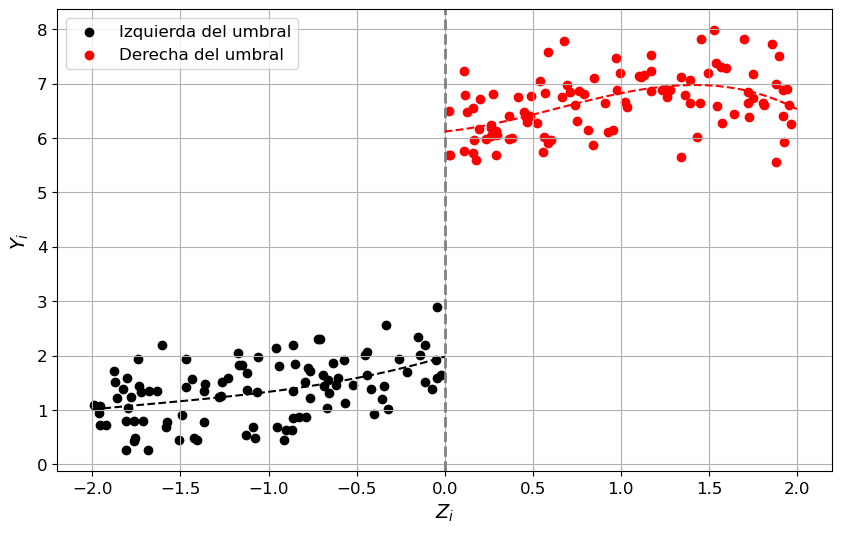
\includegraphics[width=9cm, height=9cm, keepaspectratio]{Figuras/rd-salto-discontinuidad.png}
    \end{figure}
    %\pause
    \item $Y_i$ tiene una \textcolor{blue}{discontinuidad} exactamente en $\textcolor{red}{Z_0}$. 
    \item Notar que $Y_i$ puede ser una función de $Z_i$.
    \end{itemize}
\end{frame}

%%%%%%%%%%%%%%%%%%%%%%%%%%%%%%%%%%%%%%%%%%%%%%%%%%%%%%%%%%%%%%%%%%%%%%%%%%%%%%%
%%%%%%%%%%%%%%%%%%%%%%%%%%%%%%%%%%%%%%%%%%%%%%%%%%%%%%%%%%%%%%%%%%%%%%%%%%%%%%%
\section{Resultados potenciales}

\begin{frame}{Resultados potenciales}
    \begin{itemize}
    \item \textcolor{red}{Resultados potenciales}:
    \vspace{-0.75em}
    \begin{align*}
    Y_i = 
    \begin{cases}
        Y_i(1) &\hspace{0.5pt} \text{si $i$ recibe el tratamiento}\\
        Y_i(0) &\hspace{0.5pt} \text{si $i$ no recibe el tratamiento}
    \end{cases}
    \end{align*}
    %\pause
    \item \textcolor{blue}{Método de asignación:}
    \vspace{-1em}
    \begin{align*}
        D_i = 
    \begin{cases}
        1 & \text{si } Z_i \geq \textcolor{red}{Z_0}\\
        0 & \text{si } Z_i < \textcolor{red}{Z_0} 	
    \end{cases}.
    \end{align*}
    %\pause
    \item \textbf{Implicaciones:} \smallspace
        \begin{enumerate}
        \item $Y_i(0), Y_i(1)$ \textbf{no son independientes} de la asignación al tratamiento $D_i$ (Los tratados y no tratados pueden diferir sistemáticamente). \smallspace %\pause
        \item Bajo el \textbf{RDD nítido}: dado $Z_i$, los resultados potenciales son independientes de la asignación:  
        \begin{align*}
            Y_i(0),\, Y_i(1) \;\indep\; D_i \mid Z_i.        
        \end{align*}
        \end{enumerate}
    \end{itemize}
\end{frame}


\begin{frame}{Resultados potenciales y modelo de regresión}
\begin{itemize}
    \item La CEF en \textbf{ausencia de tratamiento} es:
    \begin{align*}
    \begin{split}
    \EX[Y_i(0)|Z_i] &= m(Z_i). \\
    \end{split}
    \end{align*}
    Por ahora, somos agnósticos sobre la forma funcional $m(\cdot)$. 
    \smallspace
    %\pause
    \item Estamos interesados en el efecto \textbf{CATE}:
    \begin{align*}
    \textcolor{brown}{\tau(Z_i)} \equiv \EX[Y_i(1)-Y_i(0)|Z_i].         
    \end{align*}
    %\pause
    \item El modelo que resulta es:
    \begin{align*}
    Y_i = m(Z_i) + \textcolor{brown}{\tau(Z_i)} D_i + \epsilon_i,
    \end{align*} 
    donde \(\EX[\epsilon_i \mid Z_i] = 0.\)
\end{itemize}
\end{frame}


\begin{frame}{El problema de identificación}
\begin{itemize}
    \item Consideremos comparar resultados promedio a una distancia $\eta>0$ del umbral:  \smallspace
    \begin{enumerate}
    \item $\EX[Y_i|Z_i = \textcolor{red}{Z_0}-\eta] = m(\textcolor{red}{Z_0} - \eta)$. \vspace{0.3cm}
    \item $\EX[Y_i|Z_i = \textcolor{red}{Z_0}+\eta] = m(\textcolor{red}{Z_0}+\eta) + \textcolor{brown}{\tau(Z_0+\eta)}$. \\ \vspace{0.5cm}
    \end{enumerate}	
    %\pause
    \item Si definimos \(\brown{\tau_{dif}(\eta)} \equiv \EX[Y_i|Z_i = \textcolor{red}{Z_0}+\eta] - \EX[Y_i|Z_i = \textcolor{red}{Z_0}-\eta]\), 
    \begin{align*}
    \brown{\tau_{dif}(\eta)} = \textcolor{brown}{\tau(Z_0+\eta)} + \underbrace{m(\textcolor{red}{Z_0}+\eta)-m(\textcolor{red}{Z_0}-\eta)}_{\blue{Sesgo \; de \; selección}}.
    \end{align*}
\end{itemize}
\end{frame}

%%%%%%%%%%%%%%%%%%%%%%%%%%%%%%%%%%%%%%%%%%%%%%%%%%%%%%%%%%%%%%%%%%%%%%%%%%%%%%%
%%%%%%%%%%%%%%%%%%%%%%%%%%%%%%%%%%%%%%%%%%%%%%%%%%%%%%%%%%%%%%%%%%%%%%%%%%%%%%%
\section{Continuidad local}

\begin{frame}{Continuidad local}
\begin{tcolorbox}[colback=white, title=Supuesto de identificación (RDD nítido), arc=0mm, boxrule=0.5pt, breakable]
    \vspace{-0.5em}
    \begin{align*}
        \lim_{z \to \textcolor{red}{Z_0}^{-}} \EX\!\big[Y_i(d)\mid Z_i=z\big] = \lim_{z \to \textcolor{red}{Z_0}^{+}} \EX\!\big[Y_i(d)\mid Z_i=z\big]
    \; \text{para } d\in\{0,1\}.    
    \end{align*}
    \smallskip
    De forma equivalente, \(m(\cdot)\) y \(\brown{\tau(\cdot)}\) son continuas en \(\textcolor{red}{Z_0}\).
\end{tcolorbox}
    %\pause
\begin{itemize}
    \item \textcolor{red}{Intuición:} la relación entre $Z$ y los resultados potenciales es \textbf{suave} en la vecindad del corte; cualquier salto de $Y$ en $\textcolor{red}{Z_0}$ se debe al tratamiento.
\end{itemize}
\end{frame}


\begin{frame}{Identificación}
\begin{itemize}
    \item Diferencia de medias a distancia $\eta>0$ del corte:
    \begin{align*}
        \brown{\tau_{dif}(\eta)} = \textcolor{brown}{\tau(Z_0+\eta)} + \underbrace{m(\textcolor{red}{Z_0}+\eta)-m(\textcolor{red}{Z_0}-\eta)}_{\blue{Sesgo \; de \; selección}}.
    \end{align*}		
    %\pause
     \item En el \textbf{límite}, cuando $\eta \to 0$:
    \begin{align*}
    \begin{split}
        \lim_{\eta\to 0} \brown{\tau_{dif}(\eta)} =  \textcolor{brown}{\tau(Z_0)}.
    \end{split}
    \end{align*}	
    Bajo \textbf{continuidad local}, comparar promedios justo a la izquierda y derecha de $\textcolor{red}{Z_0}$ identifica el \textbf{CATE en el umbral} de la \textit{running variable}.
\end{itemize}
\end{frame}


\begin{frame}{Identificación}
\begin{itemize}
    \item Existen dos estrategias para identificar $\textcolor{brown}{\tau(Z_0)}$: \smallspace
    %\pause
    \begin{enumerate}
        \item \textbf{Modelar la función continua} $m(Z_i)$ de forma adecuada. La idea es \textbf{separar} la \textcolor{blue}{discontinuidad en el umbral} $\textcolor{red}{Z_0}$ de la tendencia suave de $m(Z_i)$. \smallspace
        %\pause
        \item \textbf{Restringir la comparación} a unidades ubicadas \textbf{muy cerca} del corte $\textcolor{red}{Z_0}$, donde la continuidad local es más creíble. \smallspace
    \end{enumerate}
    %\pause
    \item En la práctica, los métodos de RDD combinan \textbf{ambas ideas}: aproximar la función subyacente $m(Z_i)$ y concentrar el análisis en una \textbf{ventana estrecha} alrededor del umbral.
\end{itemize}
\end{frame}


\begin{frame}{Ejemplo de RDN con \(m(Z)\) bien especificada}
\vspace{-0.75cm}
\begin{align*}
    Y_i = m(Z_i) + \textcolor{brown}{\tau} D_i + \epsilon_i
\end{align*}
\\ \vspace{-0.3cm}
\begin{figure}[H]
    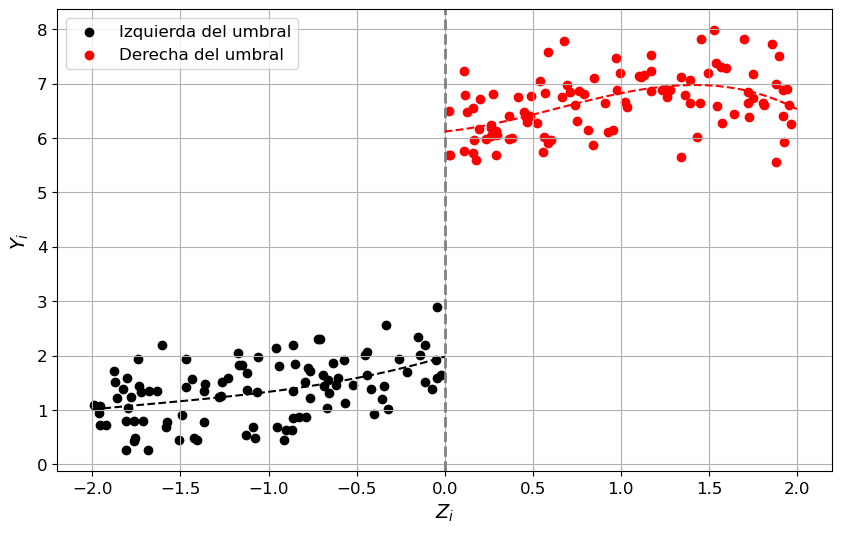
\includegraphics[width=8cm, height=8cm, keepaspectratio]{Figuras/rd-salto-discontinuidad.png}
\end{figure}
\begin{itemize}
    \item \textcolor{red}{Intuición}: MCO ajusta la tendencia continua $m(Z)$ y aísla la discontinuidad atribuible al tratamiento.
\end{itemize}
\end{frame}


\begin{frame}{Ejemplo de RDN con \(m(Z)\) mal especificada}
	\begin{figure}[H]
		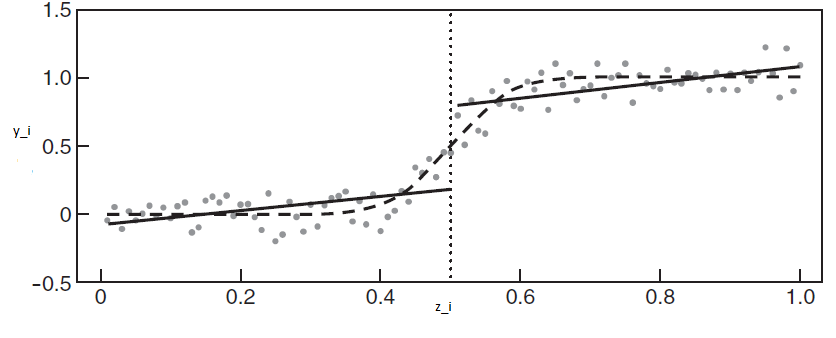
\includegraphics[width=9cm, height=9cm, keepaspectratio]{Figuras/rd-mal-especificado.png}
	\end{figure}
\begin{itemize}
    \item \textcolor{red}{Problema:} el ajuste incorrecto de $m(Z)$ puede atribuir parte de la tendencia continua al salto, generando \textbf{sesgo en la estimación}.
\end{itemize}
\end{frame}


\begin{frame}{Polinomios globales}
\begin{itemize}
    \item Una opción es aproximar $m(Z_i)$ con un \textbf{polinomio de grado} $\textcolor{olive}{P}$:
    \begin{align*}
        m(Z_i) = \beta_0 + \beta_1 Z_i + \beta_2 Z_i^2 + ... + \beta_P Z_i^P.
    \end{align*}
    %\pause
    La regresión que resulta es
    \begin{align*}
        Y_i = \beta_0 + \beta_1 Z_i + \beta_2 Z_i^2 + ... + \beta_P Z_i^P + \textcolor{brown}{\tau(Z_0)} D_i + \epsilon_i.
    \end{align*}
    %\pause
    \item \textbf{Ventaja:} entre más alto el grado $P$, mayor flexibilidad para capturar la forma de $m(Z)$. \smallspace
    \item \textbf{Problemas:}
    \begin{itemize}
        \item Estimadores menos precisos (alta varianza).
        \item Resultados muy sensibles a la elección de $P$.
        \item Riesgo de sobreajuste y oscilaciones espurias en los extremos. \smallspace
    \end{itemize}
    %\pause    
    \item Recomendación práctica: usar polinomios de \textbf{grado bajo} (\(P \leq 2\)) \citep{gelman2014high}.
\end{itemize}
\end{frame}


\begin{frame}{Restricción a la vecindad del umbral}
\begin{itemize}
    \item La idea es comparar unidades \textbf{muy cercanas} al \textcolor{blue}{umbral} $\textcolor{red}{Z_0}$. En el \textbf{límite}, cuando $\eta \to 0$:
    \[
        \lim_{\eta \to 0} \,\textcolor{brown}{\tau_{\text{dif}}(\eta)} 
        \;=\; \textcolor{brown}{\tau(Z_0)}.
    \]
    %\pause    
    \item En la práctica, aproximamos este límite restringiendo la muestra a una \textbf{ventana simétrica} alrededor de $\textcolor{red}{Z_0}$:
    \[
        Z_i \in \big[\,\textcolor{red}{Z_0}-\textcolor{olive}{h},\;\textcolor{red}{Z_0}+\textcolor{olive}{h}\,\big],
    \]
    donde $\textcolor{olive}{h}$ es el \textcolor{blue}{ancho de banda}.
    %\pause    
    \item Dentro de esa ventana, el \textbf{efecto causal local} se puede estimar como una simple \textbf{diferencia de medias} entre las observaciones a cada lado del corte.
\end{itemize}
\end{frame}


\begin{frame}{Diferencia de medias en la vecindad de $Z_0$}
\begin{figure}[H]
	 \begin{subfigure}[b]{0.48\textwidth}
	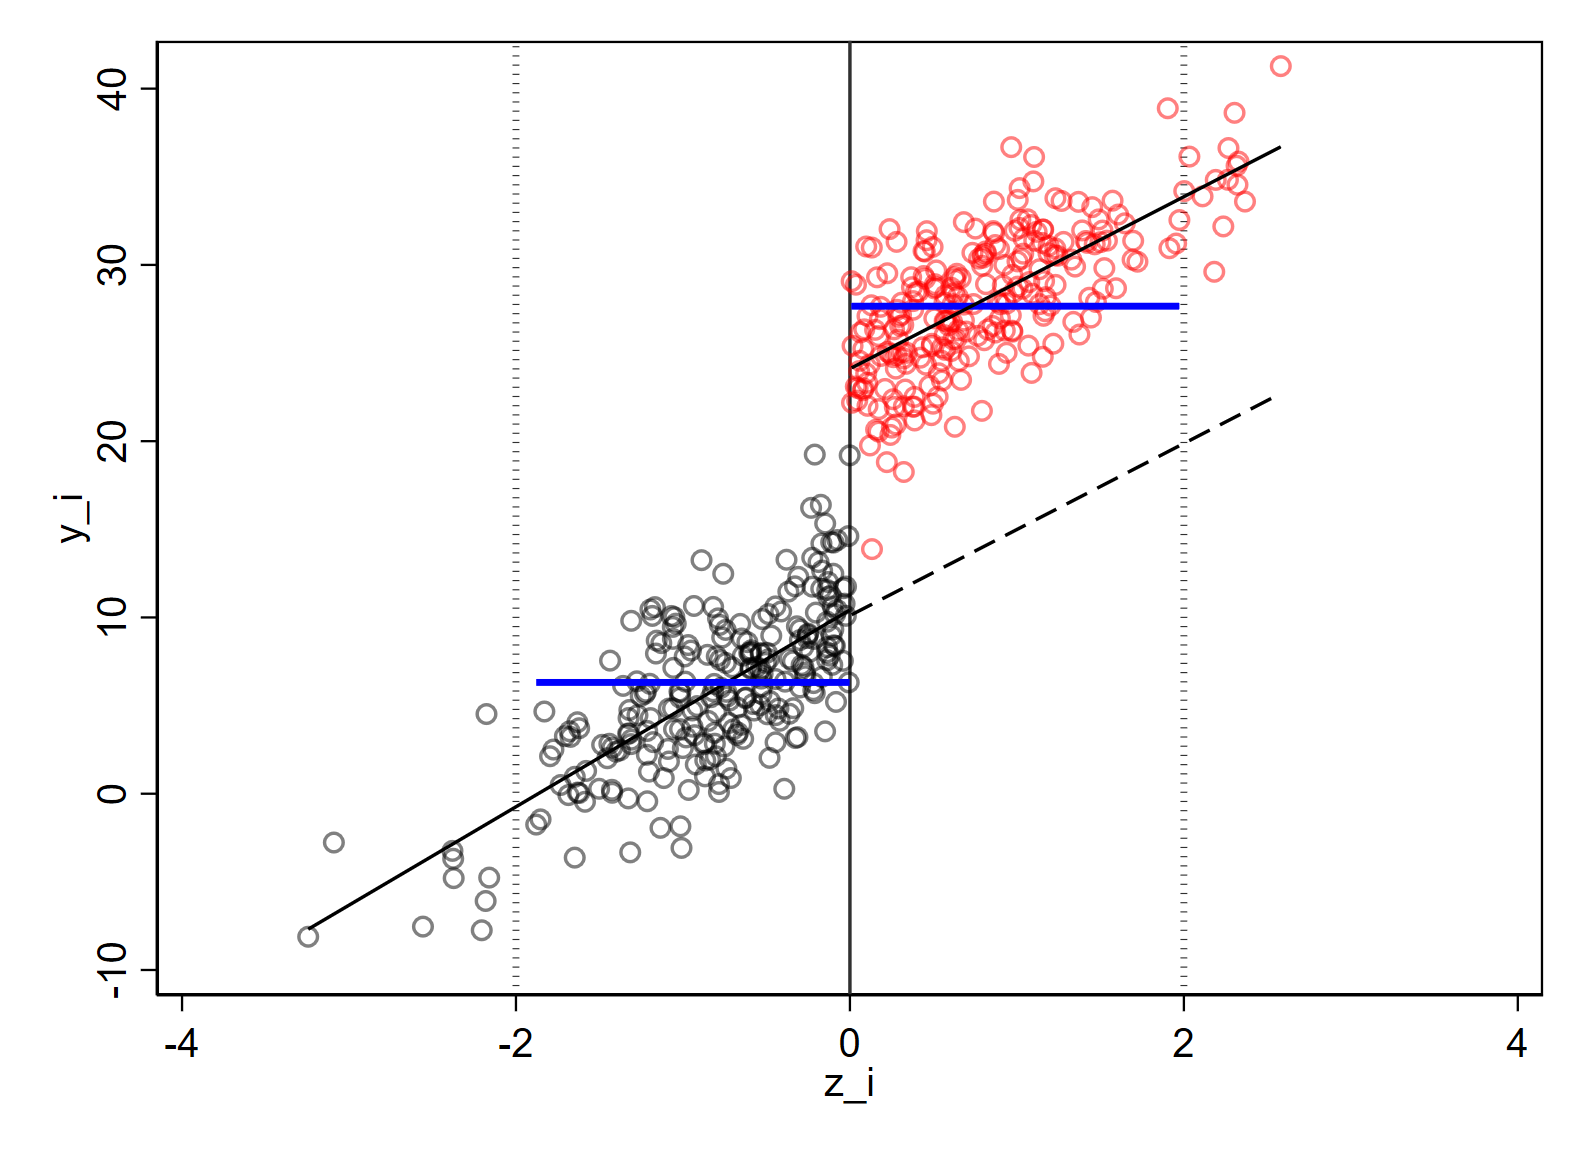
\includegraphics[width=\textwidth]{Figuras/rd-ajuste-no-parametrico-a.png}
	\end{subfigure}
	\begin{subfigure}[b]{0.48\textwidth}
	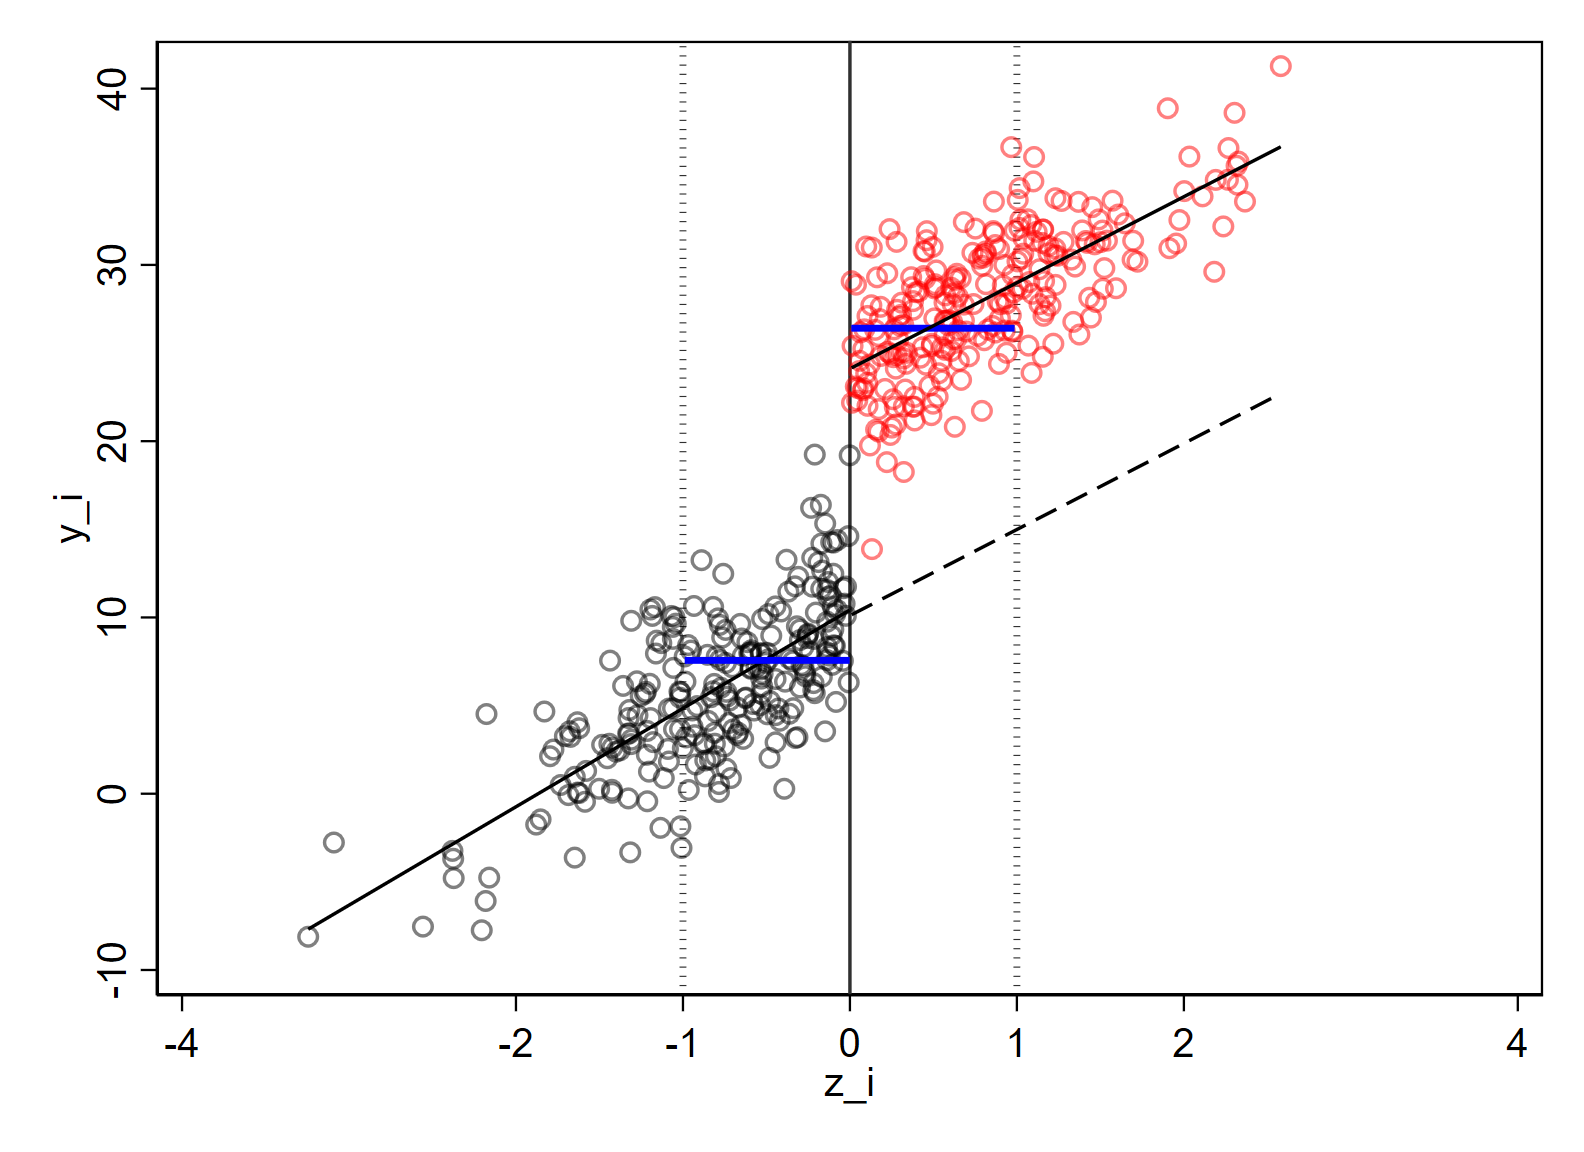
\includegraphics[width=\textwidth]{Figuras/rd-ajuste-no-parametrico-b.png}
	\end{subfigure}     
	\hfill
	\begin{subfigure}[b]{0.48\textwidth}
	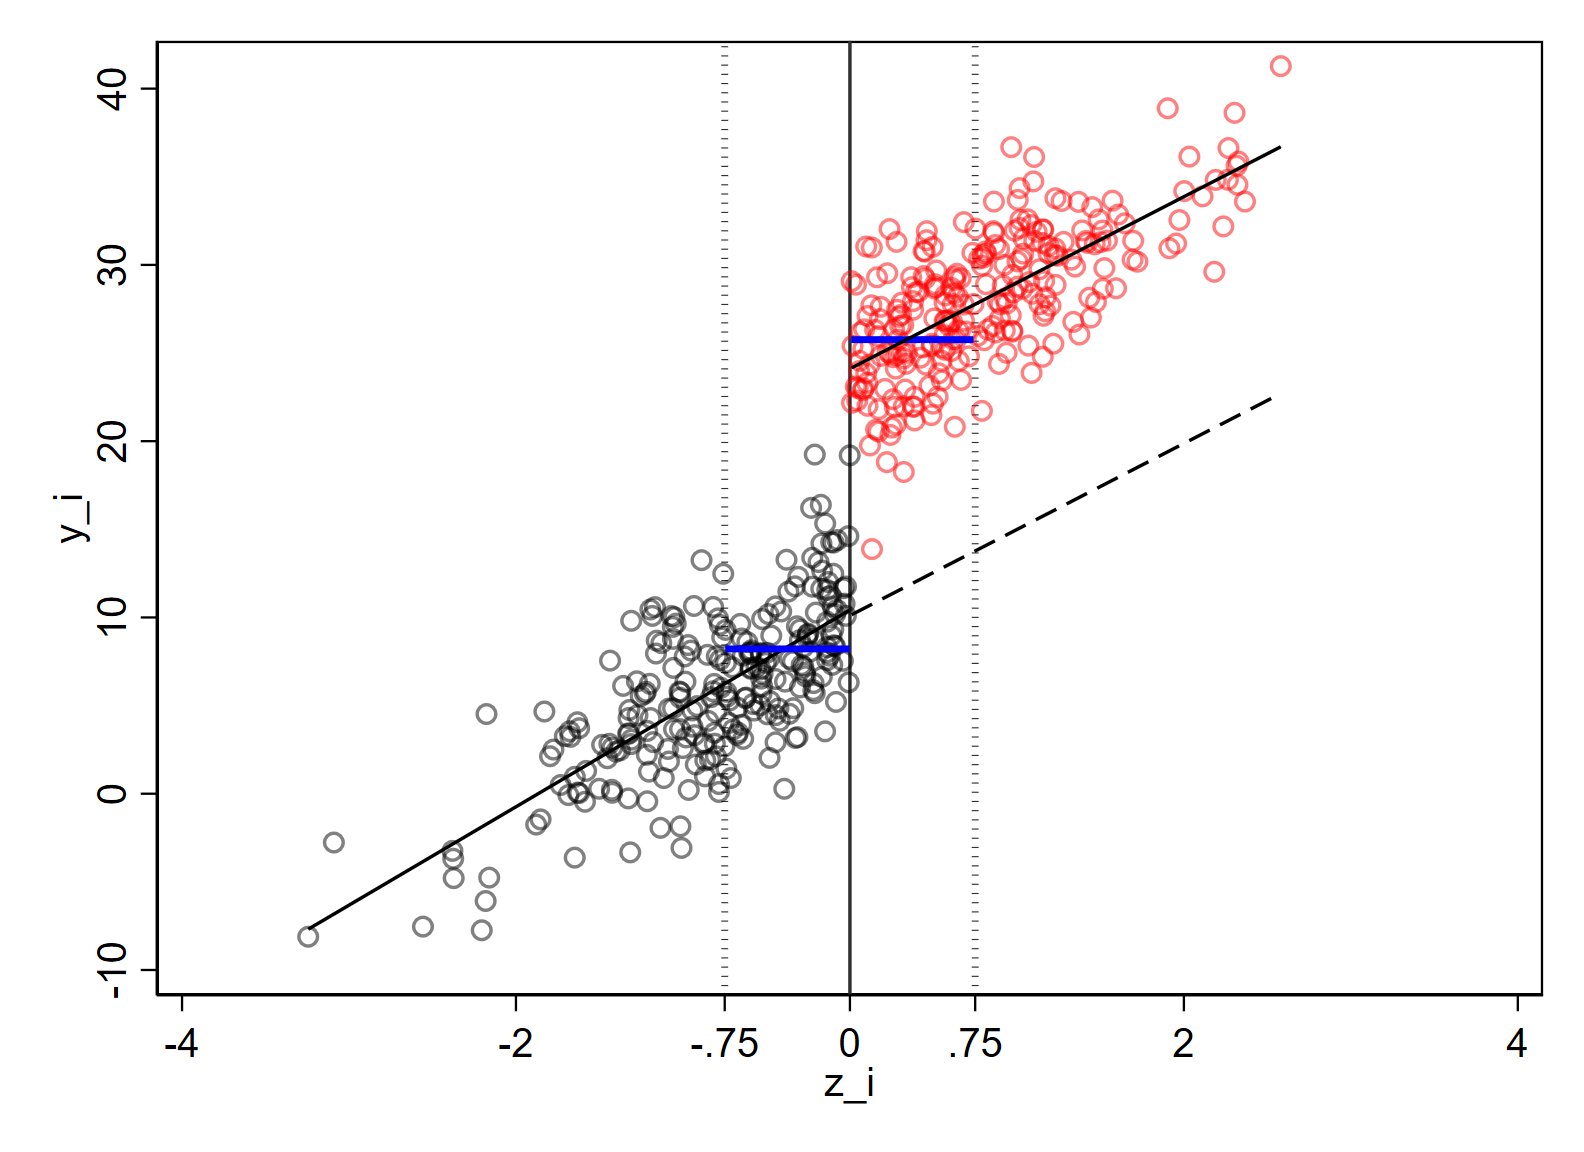
\includegraphics[width=\textwidth]{Figuras/rd-ajuste-no-parametrico-c.png}
	\end{subfigure}
\end{figure}
\end{frame}


\begin{frame}{Aleatorización local}
\begin{itemize}
    \item \textbf{Intuición:} si usamos solo las observaciones en un rango muy estrecho alrededor de $\textcolor{red}{Z_0}$, el \textcolor{blue}{sesgo de selección} desaparece en el límite: no hay selección \textbf{localmente}.
    %\pause
    \smallspace
    \item \textcolor{blue}{Aleatorización local:} los individuos justo a la izquierda y a la derecha del umbral son comparables \textcolor{red}{como si hubieran sido asignados al azar} a tratamiento y control.
    \smallspace
    %\pause
    \item Problema práctico: al reducir el ancho de banda $\textcolor{olive}{h}$, disminuye el sesgo pero también el número de observaciones $\;\Rightarrow\;$ \textbf{estimadores menos precisos}.
    %\pause
    \smallspace
     \item \textbf{Trade-off sesgo–varianza:} elegir $\textcolor{olive}{h}$ implica balancear entre reducir el sesgo (ventanas pequeñas) y mantener precisión (ventanas grandes).
\end{itemize}
\end{frame}


\begin{frame}{Regresión local: intuición}
\begin{itemize}
    \item En vez de ajustar un polinomio \textbf{global}, nos concentramos en una \textbf{ventana} alrededor del umbral $\textcolor{red}{Z_0}$. \smallspace %\pause
    \item Dentro de esa ventana: \smallspace
    \begin{itemize}
        \item Se ajusta una función $m(Z)$ sencilla (lineal o cuadrática). \smallspace 
        \item Se asignan \textbf{más peso} a las observaciones cercanas al corte, usando un kernel $K(\cdot)$. \smallspace 
    \end{itemize}
   %\pause
    \item La idea es estimar $m(Z)$ \textbf{separadamente a cada lado del umbral} y luego comparar las predicciones en $Z_0$. Esto nos da un estimador local de \textcolor{brown}{\(\tau(Z_0)\)}.
\end{itemize}
\end{frame}


\begin{frame}{Regresión local: formalización}
\begin{enumerate}
    \item Elegir el orden del polinomio ($\textcolor{olive}{P}$) y la función de pesos $K(\cdot)$. %\pause
    \item Seleccionar un ancho de banda $\textcolor{olive}{h}$ (óptimo en MSE). %\pause
    \item Estimar por \textbf{mínimos cuadrados ponderados} en cada lado de $\textcolor{red}{Z_0}$: 
\end{enumerate}
{\small
\begin{align*}
\hat{\beta}_- &= \arg\min_{\beta_{0,-},\beta_{1,-}} \sum_{i=1}^{n} \mathbf{1}[Z_i < \textcolor{red}{Z_0}] 
\left(Y_i - \beta_{0,-} - \beta_{1,-}(Z_i - \textcolor{red}{Z_0})\right)^2 
K\!\left(\frac{Z_i - \textcolor{red}{Z_0}}{\textcolor{olive}{h}}\right), \\
\hat{\beta}_+ &= \arg\min_{\beta_{0,+},\beta_{1,+}} \sum_{i=1}^{n} \mathbf{1}[Z_i \geq \textcolor{red}{Z_0}] 
\left(Y_i - \beta_{0,+} - \beta_{1,+}(Z_i - \textcolor{red}{Z_0})\right)^2 
K\!\left(\frac{Z_i - \textcolor{red}{Z_0}}{\textcolor{olive}{h}}\right).
\end{align*}
}
\[
    \textcolor{brown}{\tau(Z_0) \mid h} = \hat{\beta}_{0,+} - \hat{\beta}_{0,-}.
\]
%\pause
\begin{itemize}
    \item La inferencia requiere correcciones (e.g. \citealt{Calonico2014}).
\end{itemize}
\end{frame}


\begin{frame}{Ejemplo: \citet{lee_randomized_2008} (elecciones cerradas)}
\begin{itemize}
    \item \textbf{Pregunta:} ¿Cuál es el efecto causal de que un partido gane una elección en \(t\) sobre su probabilidad de ganar la elección siguiente (en \(t+1\))? %\pause
    \vspace{1em}
    \item \textbf{Contexto:} 
    \begin{itemize}
        \item Elecciones a la Cámara de Representantes de EE.\,UU., a nivel de distrito electoral.            
        \item Muestra: 6,558 elecciones entre 1946--1998
        \item Sistema fuertemente bipartidista: Demócratas vs. Republicanos.
    \end{itemize}
   %\pause
    \vspace{1em}
    \item \textbf{Variable de asignación:} Diferencia en el porcentaje de votos entre Demócratas y su competidor más cercano en el distrito \(i\) en el año \(t\):
    \begin{align*}
        Z_{i,t} = V^d_{i,t} - V^r_{i,t}.
    \end{align*}
\end{itemize}
\end{frame}


\begin{frame}{Diseño RDD en \citet{lee_randomized_2008}}
\begin{itemize}
    \item \textbf{Umbral:} \(\textcolor{red}{Z_0} = 0\).
    \item \textbf{Tratamiento:} ganar la elección en \(t\):
    \vspace{-1.0em}
    \begin{align*}
        D_{i,t} &= \mathbf{1}\{Z_{i,t} > 0\}.
    \end{align*}
   %\pause
    \item \textbf{Variable resultado (entre otras):}  probabilidad de ganar la elección en \(t+1\): 
    \vspace{-0.25em}
    \begin{align*}
        Y_{i,t+1} = \mathbf{1}\{V^d_{i,t+1} - V^r_{i,t+1} > 0\},
    \end{align*}   
    donde \(\mathbf{1}\{\cdot\}\) es la función indicadora.
    \vspace{1em}
    %\pause
    \item \textbf{Estimación}: regresión local alrededor del umbral (\(\textcolor{red}{Z_0}=0\)).
\end{itemize}
\end{frame}


\begin{frame}{La ventaja de la incumbencia \citep{lee_randomized_2008}}
	\begin{figure}[H]
		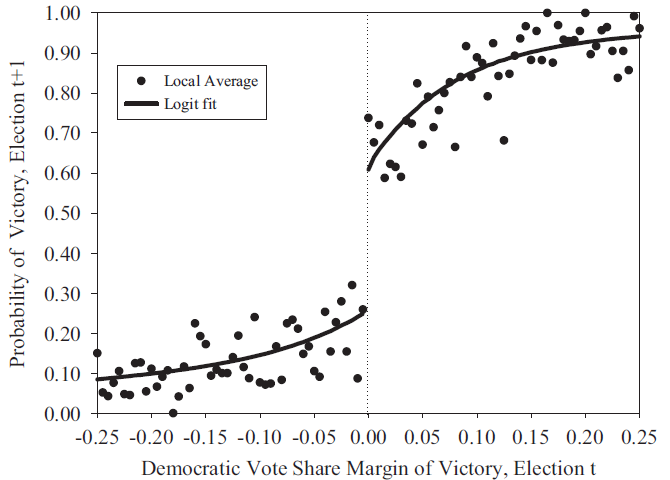
\includegraphics[width=8cm, height=8cm, keepaspectratio]{Figuras/lee2008-ventaja-incumbencia.png}
        \caption*{\scriptsize \textit{\textbf{Nota:}} Ancho de banda 0.005 (200 bins).}
	\end{figure}     
    \vspace{-0.5em}
    \begin{itemize}
        \item Si los Demócratas ganan marginalmente una elección, la probabilidad de ganar en la siguiente incrementa en \(\approx 0.4\).
    \end{itemize}
\end{frame}


%%%%%%%%%%%%%%%%%%%%%%%%%%%%%%%%%%%%%%%%%%%%%%%%%%%%%%%%%%%%%%%%%%%%%%%%%%%%%
%%%%%%%%%%%%%%%%%%%%%%%%%%%%%%%%%%%%%%%%%%%%%%%%%%%%%%%%%%%%%%%%%%%%%%%%%%%%%

\section{Validación de los supuestos y ejercicios de robustez}


\begin{frame}{Continuidad local en variables exógenas \citep{lee_randomized_2008}}
	\begin{figure}[H]
		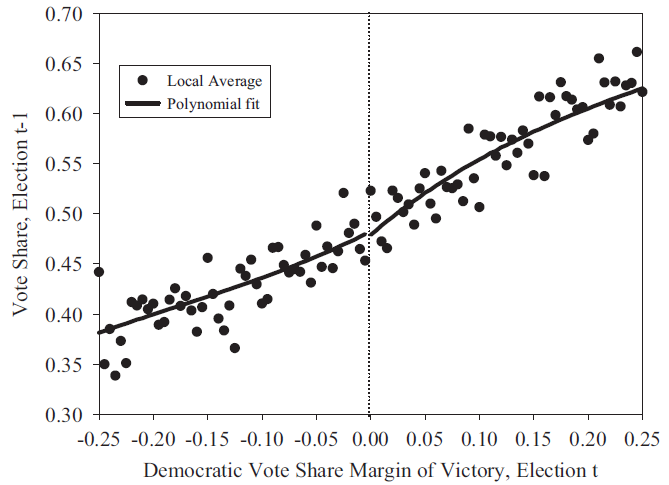
\includegraphics[width=7cm, height=7cm, keepaspectratio]{Figuras/lee2008-continuidad-variables-exogenas.png}
	\end{figure} 
\vspace{-0.4cm}
\begin{itemize}
    \item Las variables exógenas, como el margen de votación en \(t-1\), no deberían mostrar discontinuidades en el umbral \(Z_{i,t} = 0\).
\end{itemize}
\end{frame}


\begin{frame}{Manipulación de \(Z_i\) \citep{camacho_manipulation_2011}}
	\begin{figure}[H]
		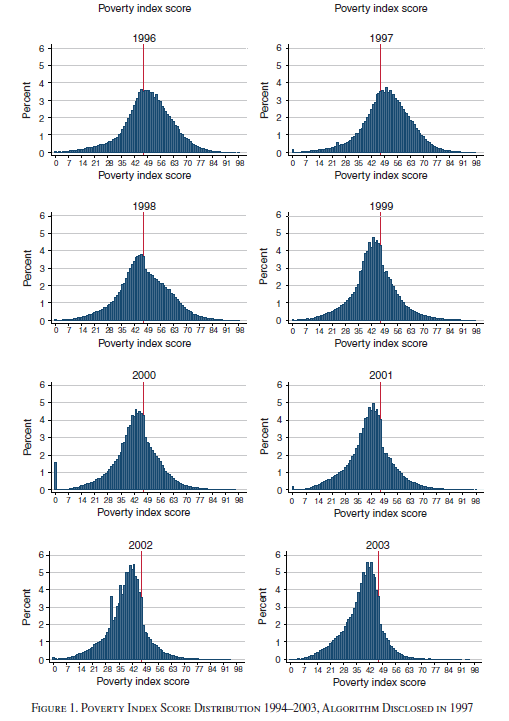
\includegraphics[width=6.5cm, height=6.5cm, keepaspectratio]{Figuras/manipulacion-densidad-camacho.png}
	\end{figure} 
\vspace{-0.4cm}
\begin{itemize}
    \item \citet{McCrary2008} propone un test estadístico para detectar manipulación: mirar si la densidad del \textit{running variable} es continua en el umbral.
\end{itemize}
\end{frame}


\begin{frame}{Robustez respecto al ancho de banda \citep{lee_randomized_2008}}
    \begin{figure}[H]
    \begin{subfigure}{.49\textwidth}
    \caption{Ancho de banda 0.001 (100 bins)}	
        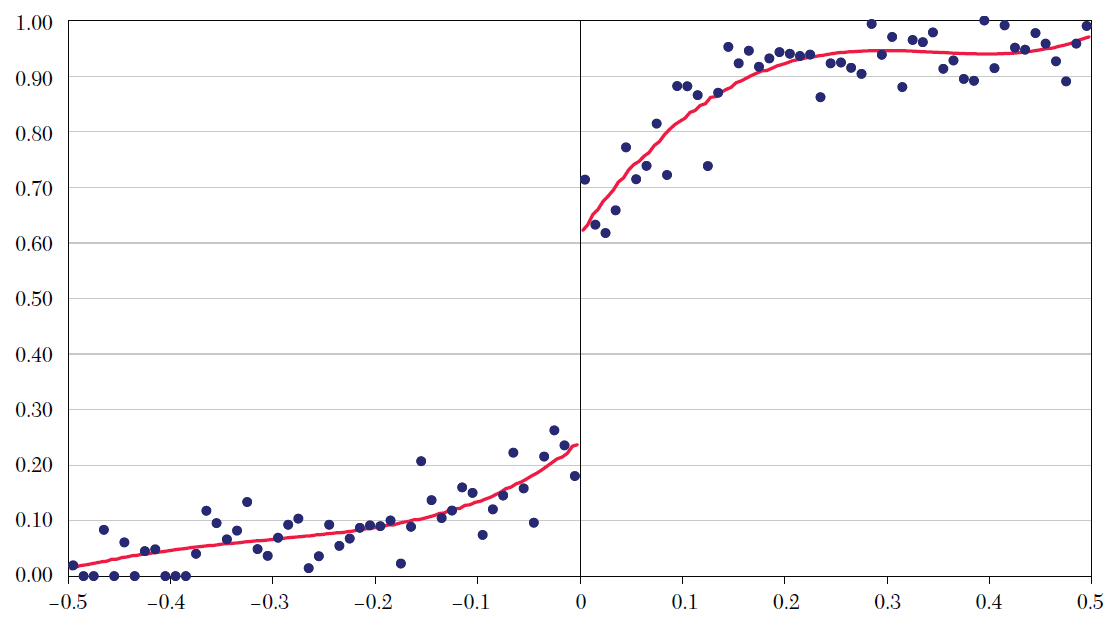
\includegraphics[width=5.5cm, height=5.5cm, keepaspectratio]{Figuras/lee2008-bandwidth-0001.png}
    \end{subfigure}
    \begin{subfigure}{.49\textwidth}
    \caption{Ancho de banda 0.02 (50 bins)}
        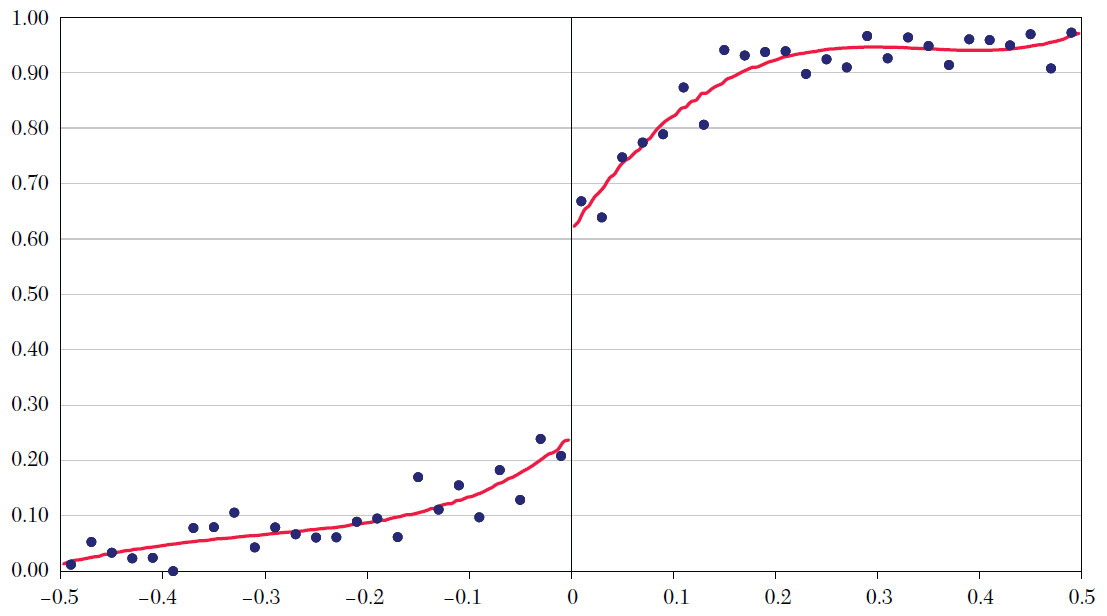
\includegraphics[width=5.5cm, height=5.5cm, keepaspectratio]{Figuras/lee2008-bandwidth-002.png}
    \end{subfigure}		
    \begin{subfigure}{.49\textwidth}
    \caption{Ancho de banda 0.005 (200 bins)}	
        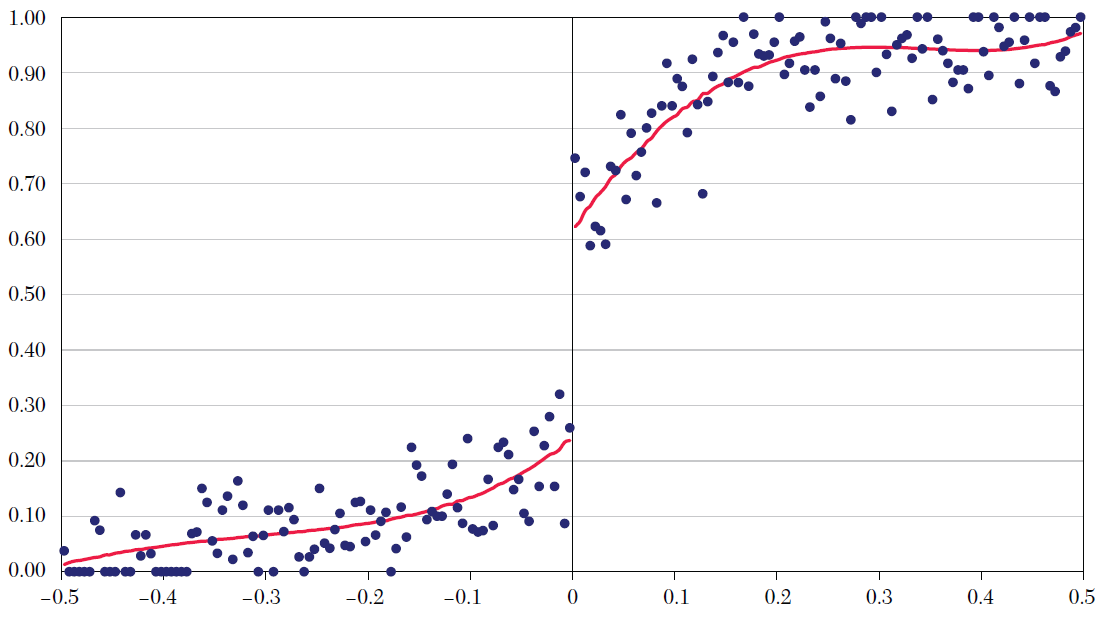
\includegraphics[width=5.5cm, height=5.5cm, keepaspectratio]{Figuras/lee2008-bandwidth-0005.png}
    \end{subfigure}
\end{figure}
\end{frame}


\begin{frame}{Extensiones}
    \begin{itemize}
        \item RD con \textbf{reglas de asignación multidimensionales} (lectura \citet{Londono-Velez2023} y \citet{Dell2010}).
        \item \textbf{RD geográfico} (lectura \citet{Dell2010}).
        \item \textbf{Regression Kink Design} (RKD) en el anexo.
    \end{itemize}
\end{frame}


%%%%%%%%%%%%%%%%%%%%%%%%%%%%%%%%%%%%%%%%%%%%%%%%%%%%%%%%%%%%%%%%%%%%%%%%%%%%%%%
%%%%%%%%%%%%%%%%%%%%%%%%%%%%%%%%%%%%%%%%%%%%%%%%%%%%%%%%%%%%%%%%%%%%%%%%%%%%%%%
\section{Anexo}

\subsection{Regression Kink Design (RKD)}

\begin{frame}{Introducción a RKD}
  \begin{itemize}
    \item \textbf{RDD} explota el \textbf{salto en la probabilidad} de recibir un tratamiento en el umbral de elegibilidad. \smallspace
   %%%\pause
    \item \textbf{RKD} explota un \textcolor{blue}{cambio en la pendiente} de la relación entre la variable de asignación ($Z$) y la variable de tratamiento ($X$) en un punto de quiebre o ``\textit{kink}'' (\textcolor{red}{$Z_0$}). \smallspace
   %%%\pause
    \begin{itemize}
        \item Cambio en la tasa marginal del impuesto sobre la renta en ciertos niveles de ingreso.
       %%%\pause
        \item Tarifas de emisión de CO2 que aumentan después de superar un límite específico. \smallspace
    \end{itemize}
   %%%\pause
    \item La idea es analizar cómo la pendiente de la relación entre la variable de resultado ($Y_i$) y la variable de asignación ($Z$) cambia en \textcolor{red}{$Z_0$}.
  \end{itemize}
\end{frame}


\begin{frame}{Cambio en la pendiente de la variable de tratamiento}
\begin{itemize}
    \item Suponga que hay un incremento en la tasa marginal de tributación a partir de un ingreso normalizado de $Z=0$.
    \vspace{-0.25em}
  \begin{figure}
    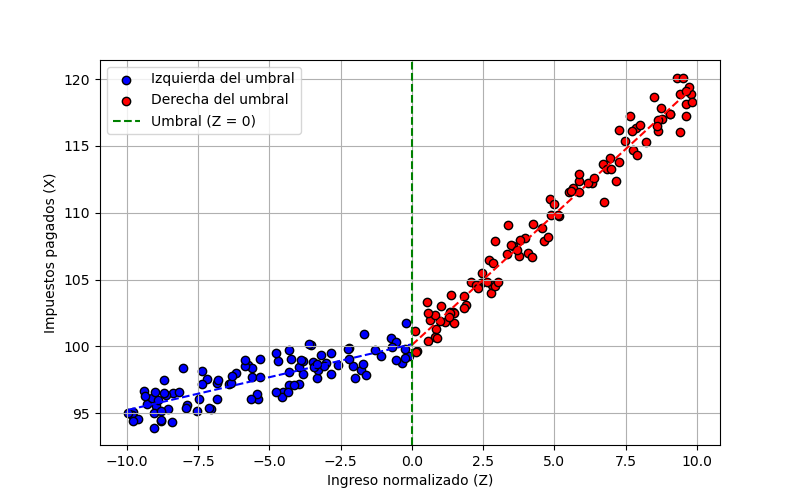
\includegraphics[width=0.8\textwidth]{Figuras/rkd-pendiente-ajustada.png}
  \end{figure}
  %%%\pause
  \item \textbf{Pregunta:} ¿El incremento en los impuestos desincentiva la oferta laboral?
\end{itemize}
\end{frame}


\begin{frame}{Cambio en la pendiente de la variable de resultado}
  \begin{figure}
    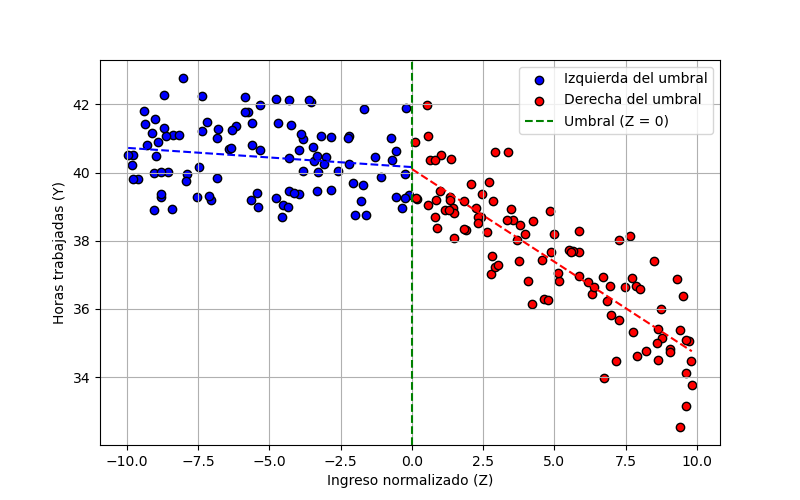
\includegraphics[width=0.85\textwidth]{Figuras/rkd-pendiente-ajustada-b.png}
  \end{figure}
 %%%%%%%%\pause
\begin{itemize}
    \item A la izquierda del punto de quiebre \textcolor{red}{\( Z_0 \)}, la relación entre ingreso y horas trabajadas tiene una pendiente negativa.
    \item Esta pendiente negativa se intensifica justo en \textcolor{red}{\( Z_0 \)}.
\end{itemize}
\end{frame}

\begin{frame}{Identificación}
    \begin{itemize}
        \item Estamos interesados en el efecto causal de un aumento en los impuestos sobre las horas trabajadas en el punto de quiebre:
        \begin{align*}
            \textcolor{orange}{\tau}(\textcolor{red}{Z_0}) \equiv \EX \left[\frac{d Y}{d X}\mid Z=\textcolor{red}{Z_0}\right]    
        \end{align*}
       %%%\pause
        \item Según \citet{Nielsen2010} y \citet{Card2012a}, bajo condiciones de regularidad:
        \begin{align*}
            \textcolor{orange}{\tau}(\textcolor{red}{Z_0}) = \frac{\lim_{\eta\to 0} \frac{d \EX[Y \vert Z=\textcolor{red}{Z_0}+\eta]}{dZ} - \lim_{\eta\to 0} \frac{d \EX[Y \vert Z=\textcolor{red}{Z_0}-\eta]}{dZ}}{\lim_{\eta\to 0} \frac{d \EX[X \vert Z=\textcolor{red}{Z_0}+\eta]}{dZ} - \lim_{\eta\to 0} \frac{d \EX[X \vert Z=\textcolor{red}{Z_0}-\eta]}{dZ}}
        \end{align*}
       %%%\pause
    \item Requerimos que cerca del umbral todo cambie ``suavemente'' excepto la derivada de la relación entre la variable de asignación y la variable de tratamiento.
    \item RKD estima el cambio en la pendiente de la respuesta, ajustado por el cambio en la pendiente de la variable de tratamiento.
    \end{itemize}
\end{frame}

\begin{frame}{Estimación (polinomio de primer orden)}
\begin{itemize}
    \item \textbf{Numerador}: \vspace{-1em}
    {\small
    \begin{align*}
\hat{\beta}_- &= \arg\min_{\beta_{0,-},\beta_{1,-}} \sum_{i=1}^{n} \mathbf{1}[Z_i < \textcolor{red}{Z_0}] \left(Y_i - \beta_{0,-} - \beta_{1,-}(Z_i - \textcolor{red}{Z_0})\right)^2 K\left(\frac{Z_i - \textcolor{red}{Z_0}}{\textcolor{olive}{h}}\right), \\
\hat{\beta}_+ &= \arg\min_{\beta_{0,+},\beta_{1,+}} \sum_{i=1}^{n} \mathbf{1}[Z_i \geq \textcolor{red}{Z_0}] \left(Y_i - \beta_{0,+} - \beta_{1,+}(Z_i - \textcolor{red}{Z_0})\right)^2 K\left(\frac{Z_i - \textcolor{red}{Z_0}}{\textcolor{olive}{h}}\right).
\end{align*}
}
%%%\pause
\item \textbf{Denominador}: \vspace{-1em}
{\small
    \begin{align*}
\hat{\gamma}_- &= \arg\min_{\gamma_{0,-},\gamma_{1,-}} \sum_{i=1}^{n} \mathbf{1}[Z_i < \textcolor{red}{Z_0}] \left(X_i - \gamma_{0,-} - \gamma_{1,-}(Z_i - \textcolor{red}{Z_0})\right)^2 K\left(\frac{Z_i - \textcolor{red}{Z_0}}{\textcolor{olive}{h}}\right), \\
\hat{\gamma}_+ &= \arg\min_{\gamma_{0,+},\gamma_{1,+}} \sum_{i=1}^{n} \mathbf{1}[Z_i \geq \textcolor{red}{Z_0}] \left(X_i - \gamma_{0,+} - \gamma_{1,+}(Z_i - \textcolor{red}{Z_0})\right)^2 K\left(\frac{Z_i - \textcolor{red}{Z_0}}{\textcolor{olive}{h}}\right).
\end{align*}
}
%%%\pause
    \item \textbf{Estimador}: \vspace{-0.5em} \[ \textcolor{orange}{\hat{\tau}}(\textcolor{red}{Z_0}) = \frac{\hat{\beta}_{1,+} - \hat{\beta}_{1,-}}{\hat{\gamma}_{1,+} - \hat{\gamma}_{1,-}}. \]
\end{itemize}
\end{frame}


% %%%%%%%%%%%%%%%%%%%%%%%%%%%%%%%%%%%%%%%%%%%%%%%%%%%%%%%%%%%%%%%%%%%%%%%%%%%%%%%
% %% Inferencia robusta: Calonico, Cattaneo y Titiunik (2014)
% %%%%%%%%%%%%%%%%%%%%%%%%%%%%%%%%%%%%%%%%%%%%%%%%%%%%%%%%%%%%%%%%%%%%%%%%%%%%%%%

% \section{Inferencia usando a \citealt{Calonico2014}}

% \begin{frame}{Inferencia en RDD: el problema}
% \begin{itemize}
%     \item El estimador de regresión local para $\textcolor{brown}{\tau(Z_0)}$ tiene la forma:
%     \[
%         \textcolor{brown}{\hat{\tau}(Z_0)} = \hat{\beta}_{0,+} - \hat{\beta}_{0,-}.
%     \]
%     %%%\pause
%     \item Con un polinomio de orden $\textcolor{olive}{P}$ y ancho de banda $\textcolor{olive}{h}$, el estimador tiene un \textbf{sesgo} (por aproximación polinomial) y una \textbf{varianza} (por muestreo). \smallspace
%     %%%\pause
%     \item El \textbf{ancho de banda óptimo en MSE} ($\textcolor{olive}{h_{\text{MSE}}}$) balancea ambos componentes:
%     \[
%         \textcolor{olive}{h_{\text{MSE}}} = \arg\min_h \;\underbrace{\text{Sesgo}^2(h)}_{\text{decrece con } h \downarrow} + \underbrace{\text{Var}(h)}_{\text{decrece con } h \uparrow}.
%     \]
%     %%%\pause
%     \item \textcolor{red}{Problema:} con $\textcolor{olive}{h_{\text{MSE}}}$, el sesgo no desaparece asintóticamente. Los \textbf{intervalos de confianza convencionales} son inválidos (cobertura real $<$ cobertura nominal).
% \end{itemize}
% \end{frame}


% \begin{frame}{Intervalos convencionales: ¿por qué fallan?}
% \begin{itemize}
%     \item El intervalo de confianza \textbf{convencional} al $95\%$ es:
%     \[
%         \text{IC}_{\text{conv}} = \textcolor{brown}{\hat{\tau}(Z_0)} \;\pm\; 1.96 \cdot \hat{\sigma}_{\text{conv}},
%     \]
%     donde $\hat{\sigma}_{\text{conv}}$ es el error estándar usual (sin corregir el sesgo). \smallspace
%     %%%\pause
%     \item Descomponemos el error del estimador:
%     \[
%         \textcolor{brown}{\hat{\tau}(Z_0)} - \textcolor{brown}{\tau(Z_0)} = \underbrace{\mathcal{B}(\textcolor{olive}{h})}_{\text{sesgo}} + \underbrace{\mathcal{V}(\textcolor{olive}{h})}_{\text{error estocástico}}.
%     \]
%     %%%\pause
%     \item Cuando usamos $\textcolor{olive}{h_{\text{MSE}}}$:
%     \begin{enumerate}
%         \item El sesgo $\mathcal{B}(\textcolor{olive}{h_{\text{MSE}}})$ es del \textbf{mismo orden} que la desviación estándar. \smallspace
%         \item El estadístico $t$ convencional \textbf{no converge} a una normal estándar:
%         \[
%             t_{\text{conv}} = \frac{\textcolor{brown}{\hat{\tau}(Z_0)} - \textcolor{brown}{\tau(Z_0)}}{\hat{\sigma}_{\text{conv}}} \;\not\to\; \mathcal{N}(0,1).
%         \]
%     \end{enumerate}
%     %%%\pause
%     \item Resultado: los IC convencionales con $\textcolor{olive}{h_{\text{MSE}}}$ tienden a \textbf{subcobertura}.
% \end{itemize}
% \end{frame}


% \begin{frame}{Corrección de sesgo \citep{Calonico2014}}
% \begin{itemize}
%     \item \textbf{Idea:} estimar el sesgo $\mathcal{B}(\textcolor{olive}{h})$ y restarlo del estimador original. \smallspace
%     %%%\pause
%     \item Para un estimador de regresión local de orden $\textcolor{olive}{P}$, el sesgo principal depende de las derivadas de orden $\textcolor{olive}{P}+1$ de $m(Z)$ evaluadas en $\textcolor{red}{Z_0}$. \smallspace
%     %%%\pause
%     \item Estas derivadas se pueden estimar ajustando un polinomio de orden $\textcolor{olive}{P}+1$ (con un ancho de banda piloto $\textcolor{olive}{b}$). \smallspace
%     %%%\pause
%     \item Estimador \textbf{corregido por sesgo}:
%     \[
%         \textcolor{brown}{\hat{\tau}_{\text{bc}}(Z_0)} = \textcolor{brown}{\hat{\tau}(Z_0)} - \hat{\mathcal{B}}(\textcolor{olive}{h}).
%     \]
%     %%%\pause
%     \item \textcolor{red}{Caso particular:} si $\textcolor{olive}{P}=1$ (regresión local lineal) y $\textcolor{olive}{h}=\textcolor{olive}{b}$, la corrección de sesgo equivale a estimar una \textbf{regresión local cuadrática} ($\textcolor{olive}{P}=2$).
% \end{itemize}
% \end{frame}


% \begin{frame}{Inferencia robusta \citep{Calonico2014}}
% \begin{itemize}
%     \item El estimador corregido $\textcolor{brown}{\hat{\tau}_{\text{bc}}(Z_0)}$ elimina el sesgo dominante, pero introduce \textbf{variabilidad adicional} (la estimación de $\hat{\mathcal{B}}$ es ruidosa). \smallspace
%     %%%\pause
%     \item \citet{Calonico2014} derivan un nuevo estimador de varianza $\hat{\sigma}_{\text{rb}}^2$ que incorpora:
%     \begin{enumerate}
%         \item La varianza del estimador original. \smallspace
%         \item La varianza adicional por la estimación del sesgo. \smallspace
%     \end{enumerate}
%     %%%\pause
%     \item El \textbf{intervalo de confianza robusto} es:
%     \[
%         \text{IC}_{\text{rb}} = \textcolor{brown}{\hat{\tau}_{\text{bc}}(Z_0)} \;\pm\; z_{\alpha/2} \cdot \hat{\sigma}_{\text{rb}}.
%     \]
%     %%%\pause
%     \item El estadístico $t$ robusto sí converge a una normal estándar:
%     \[
%         t_{\text{rb}} = \frac{\textcolor{brown}{\hat{\tau}_{\text{bc}}(Z_0)} - \textcolor{brown}{\tau(Z_0)}}{\hat{\sigma}_{\text{rb}}} \;\xrightarrow{d}\; \mathcal{N}(0,1).
%     \]
%     \item Esto es válido \textbf{incluso utilizando} $\textcolor{olive}{h_{\text{MSE}}}$.
% \end{itemize}
% \end{frame}


% \begin{frame}{Resumen: implementación práctica \citep{Calonico2014}}
% \begin{enumerate}
%     \item \textbf{Elegir} el orden del polinomio $\textcolor{olive}{P}$ (usualmente $\textcolor{olive}{P}=1$). \smallspace
%     %%%\pause
%     \item \textbf{Seleccionar} el ancho de banda $\textcolor{olive}{h_{\text{MSE}}}$ usando el selector óptimo en MSE. \smallspace
%     %%%\pause
%     \item \textbf{Estimar} $\textcolor{brown}{\hat{\tau}(Z_0)}$ por regresión local de orden $\textcolor{olive}{P}$. \smallspace
%     %%%\pause
%     \item \textbf{Estimar el sesgo} $\hat{\mathcal{B}}(\textcolor{olive}{h})$ usando un polinomio de orden $\textcolor{olive}{P}+1$ (con ancho de banda piloto $\textcolor{olive}{b}$). \smallspace
%     %%%\pause
%     \item \textbf{Construir} el estimador corregido: $\;\textcolor{brown}{\hat{\tau}_{\text{bc}}(Z_0)} = \textcolor{brown}{\hat{\tau}(Z_0)} - \hat{\mathcal{B}}(\textcolor{olive}{h})$. \smallspace
%     %%%\pause
%     \item \textbf{Reportar} intervalos de confianza \textbf{robustos} usando $\hat{\sigma}_{\text{rb}}$. \smallspace
% \end{enumerate}
% %%%\pause
% \vspace{0.3cm}
% \begin{tcolorbox}[colback=white, arc=0mm, boxrule=0.5pt]
%     \textbf{Software:} paquete \texttt{rdrobust} en R y Stata.
%     \begin{itemize}
%         \item \texttt{rdrobust}: estimación puntual e IC robustos.
%         \item \texttt{rdbwselect}: selección óptima de $\textcolor{olive}{h}$.
%         \item \texttt{rdplot}: gráficos de RDD.
%     \end{itemize}
% \end{tcolorbox}
% \end{frame}


%%%%%%%%%%%%%%%%%%%%%%%%%%%%%%%%%%%%%%%%%%%%%%%%%%%%%%%%%%%%%%%%%%%%
%%%%%%%%%%%%%%%%%%%%%%%%%%%%%%%%%%%%%%%%%%%%%%%%%%%%%%%%%%%%%%%%%%%%
%BIBLIOGRAPHY
\nobibliography{references}
\end{document}